\documentclass[11pt]{article}

\usepackage{amsmath,amssymb,amsthm}
\usepackage{hyperref}
\usepackage{enumitem}
\usepackage{geometry,comment}
\usepackage{xcolor}
\usepackage[normalem]{ulem}
\geometry{margin=1in}
\usepackage{tikz}
\usepackage{tikz-cd}
\usepackage{pgfplots}
\usepackage[binary-units=true]{siunitx}
\usepackage{graphicx}
\usepackage[font=small]{caption}
\usepackage[most]{tcolorbox}

\title{A Vanilla zkVM Architecture}
\author{George Kadianakis\quad Dmitry Khovratovich\quad Benedikt Wagner\quad Arantxa Zapico\\[8pt]
{\normalsize Ethereum Foundation Cryptography Research}}

\input{macros.tex}
\begin{document}

\maketitle

\begin{instruction}
This document is a reference example illustrating the expected scope and level of rigor. It is not meant to describe a zkVM that is implementable and efficient, and the described zkVM may not even be sound (we provide a best-effort security proof in Section~\ref{sec:security} that has not been peer-reviewed and (over-)idealizes certain aspects). Submitted documents should provide additional detail where applicable.
\end{instruction}

\section*{Overview}

This document describes a sample \emph{vanilla zkVM} architecture designed according to the W1 deliverable of the EF zkVM whitepaper guidelines\footnote{\url{https://zkevm.ethereum.foundation/blog/cryptography-research-update}}.
The architecture proves execution of a fixed RV+ (extended RISC-V) guest program using:

\begin{itemize}
\item Segmented execution traces
\item Specialized constraint systems (``chips'')
\item A system of interaction buses
\item In-circuit bus-membership checks for bus consistency
\item Abstract knowledge-sound SNARKs for all circuits
\item Recursive aggregation of segment proofs
\end{itemize}

After execution, the trace is divided into segments. Each segment is proven by four inner circuits tied together by a shared bus, whose proofs are verified by a single segment circuit. Segment proofs are then recursively aggregated in a binary tree until a single proof attests to correctness of the entire program execution.


\section{Execution Model}
We define how a program is executed.

\subsection{Program, Execution, and VM State}

A \textbf{program} $\PPP$ is a fixed RV+ binary, compiled from an Ethereum State Transition function.
Its inputs $\III$ are derived from the Ethereum state (\emph{initial state}), and
the execution witness $\WWW$,
and its outputs $\OOO$ are the final Ethereum state (\emph{final state}).

The program $\PPP$ operates on the \textbf{VM state} $S$, defined as concatenation of the following components:
\begin{itemize}
\item $\pc$: 32-bit program counter
\item $\regs[0..k-1]$: list of $k$ 32-bit register values
\item $\mem[]$: byte-addressed writable memory
\end{itemize}
We separately denote the code of the program by $\code$. It is immutable and read-only, and is not part of the VM state.

A single instruction step of the program execution is defined as a transition from
one VM state to another according to the semantics of the instruction $\op$ retrieved from
$\code$ at the program counter $\pc_1$. This is denoted as follows:
\begin{equation}\label{eq:op}
S:=(\pc_1,\regs_1,\mem_1)\xrightarrow{\op:=\code[\pc_1]} S':=(\pc_2,\regs_2,\mem_2)
\end{equation}
For example, if $\op$ is an addition instruction, which adds the first two registers and stores in the third register, then the semantics of the step is defined as
\begin{align}
\pc_2&=\pc_1+1,\\
\regs_2&=\regs_1\text{ except that } \regs_2[2]:=\regs_1[0]+\regs_1[1],\\
\mem_2&=\mem_1.
\end{align}
We will use the notation $(\pc_1,\regs_1,\mem_1)\rightarrow  (\pc_2,\regs_2,\mem_2)$ to denote that $S$ transitions to $S'$ by executing instruction
 $\op:=\code[\pc_1]$.


An \textbf{execution trace} for program $\code$ applied to inputs $\III$ is a sequence of VM states

\[
\TTT:\quad S_0 \rightarrow S_1 \rightarrow \cdots \rightarrow S_T
\]
where each step corresponds to execution of one instruction.


A \textbf{zkVM proof} for $(\PPP,\EE,\EE')$,
where $\EE$ and $\EE'$ are the initial and final Ethereum states, is a SNARK that proves the following:
$$
\begin{cases}
S_0\rightarrow\cdots\rightarrow S_T;\\
S_0:=(\pc_0:=0,\regs,\mem)\text{ where $\regs,\mem$ are derived from }\EE;\\
S_T:=(\pc_T,\regs',\mem')\text{ where $\regs',\mem'$ are derived from }\EE';\\
\end{cases}
$$

\subsection{Supported Instructions}
The zkVM supports the RV+ instruction set, which is an extension of the RV32IM instruction set.
Concretely, all operations:
\begin{itemize}
    \item conform to the state transition \eqref{eq:op}, i.e.
    transform $(\pc_1,\regs_1,\mem_1)$ to $(\pc_2,\regs_2,\mem_2)$ according to the semantics of the instruction $\op$ retrieved from $\code$ at the program counter $\pc_1$.
    \item are all standard RISC-V instructions\footnote{\url{https://riscv.org/technical/specifications/}} (executed according to the standard RISC-V semantics)
     or additional
    instructions (precompiles) for efficient execution of certain operations --- concretely,
    Keccak and Poseidon.
\end{itemize}
For our purpose the exact semantics of the instructions is not important,
and we treat them as black boxes with their own predicates modeling the correctness of the execution.

Concretely, for given instruction $op$, the predicate $\varphi_{op}$  has the semantics
\begin{multline}\label{eq:phiop}
\varphi_{op}(\pc_1,\regs_1,\mem_1,\pc_2,\regs_2,\mem_2)=\mathrm{TRUE} \;\Longleftrightarrow\;\\
 (\pc_1,\regs_1,\mem_1)\xrightarrow{\op} (\pc_2,\regs_2,\mem_2) \wedge \code[\pc_1]=op
\end{multline}

For instance, if $op$ is an ADD instruction, then $\mem_1=\mem_2$, $\pc_1+1=\pc_2$ and the registers change according to the ADD instruction.


 Exceptions are memory operations,
which we assume have the following syntax and semantics:
\begin{align}
\rea:\;&(\regs_1:=(addr,*,\ldots),\mem)\rightarrow (\regs_2:=(addr,x,\ldots),\mem),\notag\\
&\quad \mem[addr]=x,\label{eq:mem-op-read}\\
\writ:\;&(\regs_1:=(addr,x,\ldots),\mem)\rightarrow (\regs_2:=(addr,x,\ldots),\mem'),\notag\\
&\quad \mem'[i]=\begin{cases}
x & \text{if }i=addr,\\
\mem[i] & \text{otherwise}.
\end{cases}\label{eq:mem-op-write}
\end{align}

We decompose each memory predicate into a pc-and-register component
(independent of memory) and an explicit memory-access equation:
\begin{multline}
  \varphi_{\rea}(S_1,S_2) :=
    \varphi'_{\rea}(\pc_1,\regs_1,\pc_2,\regs_2)
    \;\wedge\; \mem_1[\regs_1[0]] = \regs_2[1]
    \;\wedge\; \mem_2 = \mem_1
  \label{eq:phi-read-decomp}
\end{multline}
\begin{multline}
  \varphi_{\writ}(S_1,S_2) :=
    \varphi'_{\writ}(\pc_1,\regs_1,\pc_2,\regs_2)
    \;\wedge\; \mem_2 = \mem_1[\regs_1[0]\mapsto\regs_1[1]]
  \label{eq:phi-write-decomp}
\end{multline}
where $\regs_1[0]$ denotes the address register, $\regs_1[1]$ (resp.\ $\regs_2[1]$)
the value register before (resp.\ after) the step, and
$\varphi'_{\rea}$, $\varphi'_{\writ}$ depend only on $\pc$ and $\regs$.
Both $\varphi'_{\rea}$ and $\varphi'_{\writ}$ include the well-formedness
conjunct $\regs_1[0]\in[n]$, where $n$ is the number of addressable memory
cells: without it the expressions $\mem_1[\regs_1[0]]$ and
$\mem_1[\regs_1[0]\mapsto\regs_1[1]]$ above would be undefined.  The conjunct is
memory-free, so it is inherited verbatim by the committed-memory versions of the
two predicates, and it is what lets the security proof treat $\regs_1[0]$ as a
legal index of the committed vector.

Every pc-and-register part $\varphi'_{op}$ --- of memory and non-memory
operations alike --- also carries the fetch conjunct $\code[\pc_1]=op$
of~\eqref{eq:phiop}; the conjunct depends only on $\pc_1$ (the code $\code$ is
fixed), so it is memory-free and belongs in $\varphi'_{op}$.  This placement is
load-bearing: the security analysis (Remark~\ref{rem:mem-ext-hyp4}) relies on
it to conclude that at most one operation's disjunct of the step predicate can
hold, and that this operation is $\code[\pc_1]$.
\begin{instruction}
Teams whose architecture selects the operation differently (e.g.\ via selector
columns) must ensure an equivalent guarantee: the constraint system must force
the satisfied operation branch to be the one fetched at $\pc_1$.  Without it,
the memory-reconstruction rule of
Proposition~\ref{prop:memory-extractability} can diverge from the satisfied
branch and the commitment invariant fails without any binding violation.
\end{instruction}

The conjunct $\mem_2=\mem_1$ in~\eqref{eq:phi-read-decomp} is kept explicit for
the same reason as for the non-memory operations: a read must not be able to
silently alter memory.  Without it $\varphi_{\rea}$ would leave $\mem_2$ completely
unconstrained, and a trace satisfying $\varphi_{\step}$ at every step could
still replace the whole memory at a read.  Note that $\varphi_{\writ}$ needs no
such conjunct, as~\eqref{eq:phi-write-decomp} already determines $\mem_2$
entirely.



\section{Segmentation}
We now explain how execution is split into segments.

\subsection{Execution Segments}

\begin{figure}
\centering
\resizebox{0.99\textwidth}{!}{%
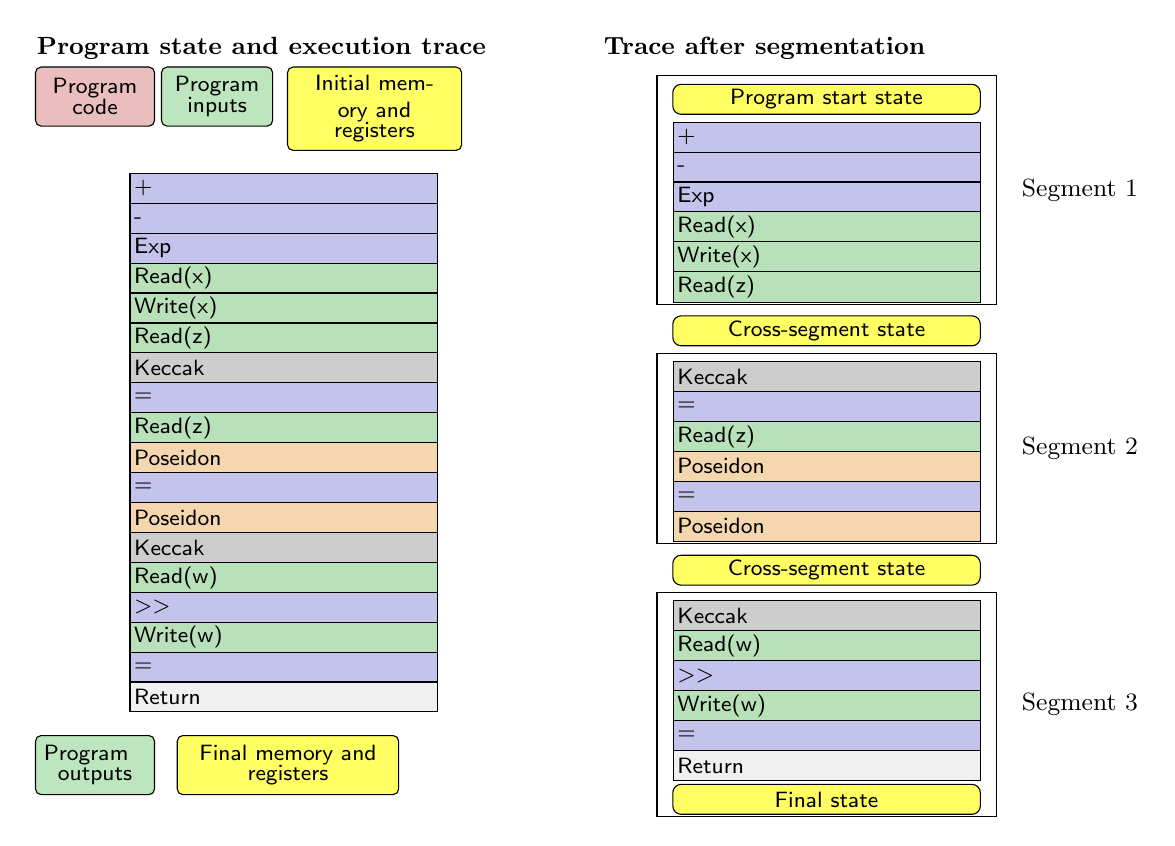
\begin{tikzpicture}[y=-1cm]
  % Colors
  \definecolor{alucol}{RGB}{195,195,235}
  \definecolor{memcol}{RGB}{185,225,185}
  \definecolor{hashcol}{RGB}{205,205,205}
  \definecolor{poscol}{RGB}{245,215,175}
  \definecolor{retcol}{RGB}{240,240,240}
  \definecolor{codecol}{RGB}{235,190,190}
  \definecolor{inputcol}{RGB}{190,230,190}
  \definecolor{statecol}{RGB}{255,255,100}
  %
  \def\rh{0.38}
  \def\bw{3.8cm}
  %
  \tikzset{
    ibox/.style={draw, thin, minimum height=\rh cm, text width=\bw, inner sep=1.5pt,
                 anchor=north west, font=\footnotesize\sffamily},
    sbox/.style={draw, thin, rounded corners=3pt, fill=statecol, minimum height=0.38cm,
                 text width=\bw, align=center, inner sep=1.5pt, font=\footnotesize\sffamily,
                 anchor=north},
    tbox/.style={draw, thin, rounded corners=2pt, minimum height=0.75cm, inner sep=3pt,
                 font=\footnotesize\sffamily, align=center, anchor=north west},
    seglabel/.style={font=\small, anchor=west},
  }
  %
  %%% LEFT SIDE %%%
  \node[anchor=north west, font=\small\bfseries] at (0, 0) {Program state and execution trace};
  %
  % Top boxes
  \node[tbox, fill=codecol, text width=1.3cm] at (0.1, 0.5) {Program\\[-2pt]code};
  \node[tbox, fill=inputcol, text width=1.2cm] at (1.7, 0.5) {Program\\[-2pt]inputs};
  \node[tbox, fill=statecol, text width=2.0cm] at (3.3, 0.5) {Initial memory and\\[-2pt]registers};
  %
  % Left instruction list (18 rows)
  \def\ly{1.85}
  \def\lx{1.3}
  \foreach \n/\txt/\col in {
    0/{+}/alucol, 1/{-}/alucol, 2/{Exp}/alucol,
    3/{Read(x)}/memcol, 4/{Write(x)}/memcol, 5/{Read(z)}/memcol,
    6/{Keccak}/hashcol, 7/{=}/alucol, 8/{Read(z)}/memcol,
    9/{Poseidon}/poscol, 10/{=}/alucol, 11/{Poseidon}/poscol,
    12/{Keccak}/hashcol, 13/{Read(w)}/memcol,
    14/{\textgreater\textgreater}/alucol, 15/{Write(w)}/memcol,
    16/{=}/alucol, 17/{Return}/retcol%
  } {
    \node[ibox, fill=\col] at (\lx, {\ly+\n*\rh}) {\txt};
  }
  %
  % Bottom boxes
  \node[tbox, fill=inputcol, text width=1.3cm] at (0.1, {\ly+18*\rh+0.3}) {\raggedright Program\\[-2pt]outputs};
  \node[tbox, fill=statecol, text width=2.6cm] at (1.9, {\ly+18*\rh+0.3}) {Final memory and\\[-2pt]registers};
  %
  %%% RIGHT SIDE %%%
  \def\rx{8.2}
  \pgfmathsetmacro{\rcx}{\rx + 1.953}
  %
  \node[anchor=north west, font=\small\bfseries] at (7.2, 0) {Trace after segmentation};
  %
  % --- Segment 1 ---
  \def\startY{0.72}
  \node[sbox] at (\rcx, \startY) {Program start state};
  %
  \pgfmathsetmacro{\segAy}{\startY + 0.48}
  \foreach \n/\txt/\col in {
    0/{+}/alucol, 1/{-}/alucol, 2/{Exp}/alucol,
    3/{Read(x)}/memcol, 4/{Write(x)}/memcol, 5/{Read(z)}/memcol%
  } {
    \node[ibox, fill=\col] at (\rx, {\segAy+\n*\rh}) {\txt};
  }
  %
  \pgfmathsetmacro{\segAtop}{\startY - 0.1}
  \pgfmathsetmacro{\segAbot}{\segAy + 6*\rh + 0.04}
  \draw[thin] ({\rx-0.2}, \segAtop) rectangle ({\rx+3.8+0.11+0.2}, \segAbot);
  \node[seglabel] at ({\rx+3.8+0.11+0.4}, {(\segAtop+\segAbot)/2}) {Segment 1};
  %
  % --- Cross-segment state 1 ---
  \pgfmathsetmacro{\isAy}{\segAbot + 0.14}
  \node[sbox] at (\rcx, \isAy) {Cross-segment state};
  %
  % --- Segment 2 ---
  \pgfmathsetmacro{\segBy}{\isAy + 0.58}
  \foreach \n/\txt/\col in {
    0/{Keccak}/hashcol, 1/{=}/alucol, 2/{Read(z)}/memcol,
    3/{Poseidon}/poscol, 4/{=}/alucol, 5/{Poseidon}/poscol%
  } {
    \node[ibox, fill=\col] at (\rx, {\segBy+\n*\rh}) {\txt};
  }
  %
  \pgfmathsetmacro{\segBtop}{\segBy - 0.1}
  \pgfmathsetmacro{\segBbot}{\segBy + 6*\rh + 0.04}
  \draw[thin] ({\rx-0.2}, \segBtop) rectangle ({\rx+3.8+0.11+0.2}, \segBbot);
  \node[seglabel] at ({\rx+3.8+0.11+0.4}, {(\segBtop+\segBbot)/2}) {Segment 2};
  %
  % --- Cross-segment state 2 ---
  \pgfmathsetmacro{\isBy}{\segBbot + 0.14}
  \node[sbox] at (\rcx, \isBy) {Cross-segment state};
  %
  % --- Segment 3 ---
  \pgfmathsetmacro{\segCy}{\isBy + 0.58}
  \foreach \n/\txt/\col in {
    0/{Keccak}/hashcol, 1/{Read(w)}/memcol,
    2/{\textgreater\textgreater}/alucol, 3/{Write(w)}/memcol,
    4/{=}/alucol, 5/{Return}/retcol%
  } {
    \node[ibox, fill=\col] at (\rx, {\segCy+\n*\rh}) {\txt};
  }
  %
  \pgfmathsetmacro{\finalY}{\segCy + 6*\rh + 0.05}
  \node[sbox] at (\rcx, \finalY) {Final state};
  %
  \pgfmathsetmacro{\segCtop}{\segCy - 0.1}
  \pgfmathsetmacro{\segCbot}{\finalY + 0.42}
  \draw[thin] ({\rx-0.2}, \segCtop) rectangle ({\rx+3.8+0.11+0.2}, \segCbot);
  \node[seglabel] at ({\rx+3.8+0.11+0.4}, {(\segCtop+\segCbot)/2}) {Segment 3};
\end{tikzpicture}%
}
\caption{Segmentation of the execution trace into 3 segments }\label{img:trace-seg}
\end{figure}

After execution, the execution trace $\TTT$ is divided into segments $\GGG_1,\GGG_2,\ldots,\GGG_m$
of exactly $N_{\text{seg}}$ instructions\footnote{The instruction
set has a no-op instruction to pad the segment to the full length.
The parameter $N_{\text{seg}}$ is assumed to be hardcoded and fixed, and known to the verifier.} each (cf. Fig. \ref{img:trace-seg}). Each segment $\GGG_i$ corresponds to a contiguous
subsequence of the execution trace, from $S_{start_i}$ to $S_{end_i}$, and is proven by a set of separate
proofs.
The segmentation of the execution trace into consecutive segments
allows reducing the proof of the entire execution to proving the validity of each segment
and consistency between them. The global consistency argument asserts that the segments are consistent with each other
and with the public inputs/outputs:
$$
S_{end_i} = S_{start_{i+1}}\text{ for all }i\in[m-1],\quad S_{start_1}=S_0,\quad S_{end_m}=S_T.
$$

\subsection{Segment layout}

Each segment is represented in an equivalent form as a collection of one trace and several
\emph{chips}, listed below (cf.\ Fig.~\ref{img:segments}).


\paragraph{Segment trace}
It consists of all  operations of the execution trace within
the segment and state variables, including the program counter, register values, memory state, etc.
It is a collection of $N_{\text{seg}}$ rows, each corresponding to one instruction step
from the segment. The segment trace does not enforce the semantics of all instructions,
but only a subset of them, and the rest of the instructions are proven
in separate chips  and their consistency with the segment trace is enforced by
\emph{consistency arguments}.

\paragraph{Keccak chip}  It consists of all Keccak precompile calls in the segment, and their inputs/outputs.

\paragraph{Poseidon chip}
It consists of all Poseidon precompile calls in the segment, and their inputs/outputs.

\paragraph{Range check chip}
It consists of all range check statements occurring in the segment.

\paragraph{Local consistency argument}$\phantom{=}$

\begin{instruction}
  Teams should describe how their bus consistency argument works in terms of lookups used and how they integrate into the overall proof system.
\end{instruction}

The consistency arguments enforce that the operations proven in the chips are consistent
with the segment trace. This is done using the concept of a \emph{bus} connecting the segment trace and the chips,
and lookup arguments to enforce consistency of the bus values with the segment trace and the chip traces.

\begin{figure}
\centering
\resizebox{0.65\textwidth}{!}{%
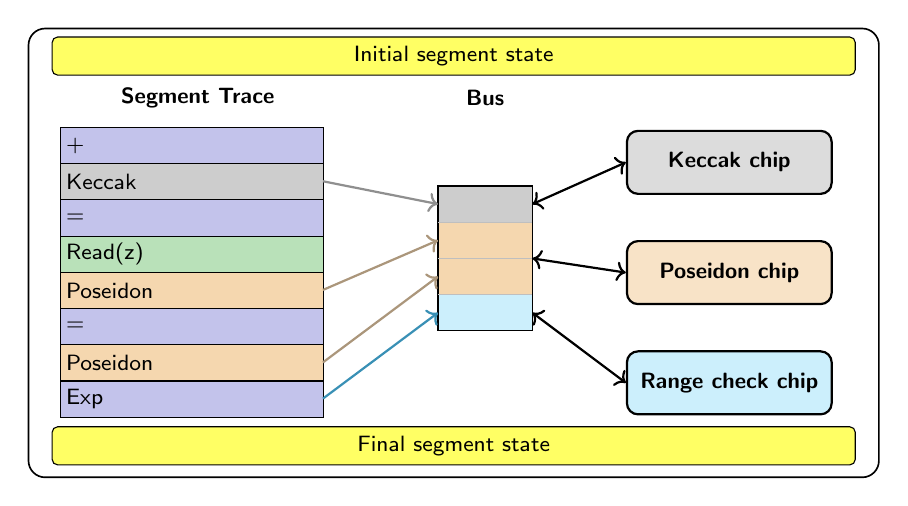
\begin{tikzpicture}[y=-1cm]
  % Colors
  \definecolor{alucol}{RGB}{195,195,235}
  \definecolor{memcol}{RGB}{185,225,185}
  \definecolor{hashcol}{RGB}{205,205,205}
  \definecolor{poscol}{RGB}{245,215,175}
  \definecolor{statecol}{RGB}{255,255,100}
  \definecolor{buscol}{RGB}{255,195,115}
  %
  \def\rh{0.46}
  %
  \tikzset{
    ibox/.style={draw, thin, minimum height=\rh cm, text width=3.2cm, inner sep=2pt,
                 anchor=north west, font=\footnotesize\sffamily},
    chip/.style={draw, thick, rounded corners=4pt, minimum width=2.6cm, minimum height=0.8cm,
                 font=\footnotesize\sffamily\bfseries, align=center},
    sbar/.style={draw, thin, rounded corners=2pt, fill=statecol,
                 minimum height=0.42cm, minimum width=10.2cm,
                 font=\footnotesize\sffamily},
  }
  %
  % Layout constants
  \def\tx{0.4}     % trace x
  \def\trw{3.34}   % trace box total width (3.2 text + 0.14 inner sep)
  \def\busx{5.2}   % bus x (shifted right for arrow space)
  \def\busw{1.2}   % bus width
  \def\ty{1.25}    % trace y start
  \def\bsy{2.0}    % bus start y (shorter than trace)
  %
  % === BIG ENCLOSING BOX ===
  \draw[semithick, rounded corners=6pt] (0, 0) rectangle (10.8, 5.7);
  %
  % === INITIAL STATE BAR ===
  \node[sbar] at (5.4, 0.35) {Initial segment state};
  %
  % === COLUMN LABELS ===
  \node[font=\footnotesize\sffamily\bfseries] at (2.15, 0.88) {Segment Trace};
  \node[font=\footnotesize\sffamily\bfseries] at ({\busx + \busw/2}, 0.88) {Bus};
  %
  % === INSTRUCTION ROWS (color-coded by chip affiliation) ===
  \foreach \n/\txt/\col in {
    0/{+}/alucol,
    1/{Keccak}/hashcol,
    2/{=}/alucol,
    3/{Read(z)}/memcol,
    4/{Poseidon}/poscol,
    5/{=}/alucol,
    6/{Poseidon}/poscol,
    7/{Exp}/alucol%
  } {
    \node[ibox, fill=\col] at (\tx, {\ty+\n*\rh}) {\txt};
  }
  %
  % === BUS COLUMN (only precompile/range-check entries, colored by chip) ===
  % 4 cells: Keccak, Poseidon, Poseidon, Range check
  \fill[hashcol]  (\busx, \bsy) rectangle ({\busx+\busw}, {\bsy+\rh});
  \fill[poscol]   (\busx, {\bsy+\rh}) rectangle ({\busx+\busw}, {\bsy+2*\rh});
  \fill[poscol]   (\busx, {\bsy+2*\rh}) rectangle ({\busx+\busw}, {\bsy+3*\rh});
  \fill[cyan!20]  (\busx, {\bsy+3*\rh}) rectangle ({\busx+\busw}, {\bsy+4*\rh});
  % Grid
  \draw[thin] (\busx, \bsy) rectangle ({\busx+\busw}, {\bsy+4*\rh});
  \foreach \n in {1,2,3} {
    \draw[thin, black!25] (\busx, {\bsy+\n*\rh}) -- ({\busx+\busw}, {\bsy+\n*\rh});
  }
  %
  % === ARROWS: TRACE → BUS ===
  \pgfmathsetmacro{\trR}{\tx + \trw}  % trace right edge
  % Keccak (trace row 1) → bus cell 0
  \draw[->, thick, hashcol!70!black] (\trR, {\ty+1*\rh+\rh/2}) -- (\busx, {\bsy+\rh/2});
  % Poseidon (trace row 4) → bus cell 1
  \draw[->, thick, poscol!70!black] (\trR, {\ty+4*\rh+\rh/2}) -- (\busx, {\bsy+\rh+\rh/2});
  % Poseidon (trace row 6) → bus cell 2
  \draw[->, thick, poscol!70!black] (\trR, {\ty+6*\rh+\rh/2}) -- (\busx, {\bsy+2*\rh+\rh/2});
  % Exp/range check (trace row 7) → bus cell 3
  \draw[->, thick, cyan!70!black] (\trR, {\ty+7*\rh+\rh/2}) -- (\busx, {\bsy+3*\rh+\rh/2});
  %
  % === FINAL STATE BAR ===
  \node[sbar] at (5.4, 5.3) {Final segment state};
  %
  % === CHIP BOXES (spread across full trace height) ===
  \node[chip, fill=hashcol!70] (sha3chip) at (8.9, 1.7) {Keccak chip};
  \node[chip, fill=poscol!70] (poschip) at (8.9, 3.1) {Poseidon chip};
  \node[chip, fill=cyan!20] (rangechip) at (8.9, 4.5) {Range check chip};
  %
  % === ARROWS: BUS → CHIPS (bidirectional) ===
  \draw[<->, thick] ({\busx+\busw}, {\bsy+\rh/2}) -- (sha3chip.west);
  \draw[<->, thick] ({\busx+\busw}, {\bsy+2*\rh}) -- (poschip.west);
  \draw[<->, thick] ({\busx+\busw}, {\bsy+3*\rh+\rh/2}) -- (rangechip.west);
  %
\end{tikzpicture}%
}
\caption{Segment structure: segment trace connects to the bus which then connects to chips.}\label{img:segments}
\end{figure}


\section{Correct execution of a program}
In this section, we define via predicates what it means that a program is correctly executed. We will use these predicates in Section~\ref{sec:proof-arch} to define the relations that the zkVM proves.

\subsection{Predicates for individual operations}

\begin{instruction}
Teams should list all operations supported by their zkVM and define the corresponding predicates based on their architecture.
\end{instruction}

Each operation is treated as a black box with its
own predicate $\varphi_{op}$ (cf. ~\eqref{eq:phiop}).
Throughout this section, subscripts $1$ and $2$ denote states before and after an operation.
We also denote $S_1:=(\pc_1,\regs_1,\mem_1)$ and
$S_2:=(\pc_2,\regs_2,\mem_2)$ as the states
before and after the operation.

We group operations as follows:
\begin{itemize}
	\item \textbf{Memory operations.}
	Read: $\pred{read}(S_1,S_2)$ --- does not modify memory.
	Write: $\pred{write}(S_1,S_2)$ --- may modify memory.
	\item \textbf{Precompiles.}
	Keccak: $\pred{keccak}(S_1,S_2)$.
	Poseidon: $\pred{poseidon}(S_1,S_2)$.
	 \item \textbf{Arithmetic without range checks.} $\op_1,\ldots,\op_{10}$
	 with predicates $
   \pred{\op_i}(S_1,S_2)$.
	 \item \textbf{Arithmetic with range checks.} $\op_{11},\ldots,\op_{20}$
	 with predicates $\pred{\op_i}(S_1,S_2)$, each decomposable as
	 $\pred{\op_i}'(S_1,S_2)\wedge \pred{range}(S_1)$
	 where the constants defining the range check are always in the
   last two registers.
\end{itemize}
All operations except $\rea$ and $\writ$ neither read nor write memory. For
such an operation we take
$\varphi_{op}(S_1,S_2) := \varphi'_{op}(\pc_1,\regs_1,\pc_2,\regs_2) \wedge \mem_2 = \mem_1$,
where $\varphi'_{op}$ depends only on $\pc$ and $\regs$ and, as for every
operation, includes the fetch conjunct $\code[\pc_1]=op$
of~\eqref{eq:phiop}; the memory-equality
conjunct $\mem_2 = \mem_1$ is kept explicit so that a non-memory step cannot
silently alter memory. We write $\varphi'_{op}$ (and its committed version) for
the pc-and-register part and keep the conjunct explicit throughout.
\subsection{Correct execution of a single step}

\begin{instruction}
Teams should define the step predicate for their architecture, specifying how the correct operation is selected and verified at each step.
\end{instruction}

A single step executes the instruction at the current program counter.
The step predicate selects the matching operation via a disjunction over all opcodes:
\begin{equation*}\label{eq:step}
\varphi_{step}(S_1,S_2):=
\bigvee_{op\in \text{operations}} \varphi_{op}(S_1,S_2)
\end{equation*}
where $S_1:=(\pc_1,\regs_1,\mem_1)$ and $S_2:=(\pc_2,\regs_2,\mem_2)$ are the states before and after the step.
Recall from~\eqref{eq:phiop} that each $\varphi_{op}$ includes the fetch conjunct
$\code[\pc_1]=op$; hence $\varphi_{step}$ binds every step to the fixed program $\code$.

\subsection{Delegating expensive operations using a Bus}

\begin{instruction}
Teams should describe how expensive operations (e.g., precompiles, range checks) are delegated to a bus or similar mechanism in their architecture.
\end{instruction}

Range checks and precompile calls are expensive to prove inline.
Instead, we collect them in a shared \emph{bus} $\BBB$
and verify separately, proving the consistency along the way.
The \emph{bus} $\BBB$ is a collection of  all
precompile calls and range checks within a segment. That is, it has the following structure:
$$
\BBB=\{(\underbrace{\op^{(i)}}_{\in\{\keccak,\poseidon\}},
S_1^{(i)},S_2^{(i)})\}_{i=1}^{b}\;\cup\;
\{(\range,S^{(j)} )\}_{j=1}^{r}
$$
where $b$ is the number of precompile calls and $r$ is the number of range checks.


Now we define auxiliary predicates that filter the bus by operation type
and assert correctness of each entry:
$\pred{\keccak}(\BBB)$ checks all Keccak entries,
$\pred{\poseidon}(\BBB)$ checks all Poseidon entries,
and $\pred{\range}(\BBB)$ checks all range-check entries.
Concretely:
\begin{align*}
\pred{\keccak}(\BBB)&:=
\bigwedge_{( \keccak,S_1,S_2)\in\BBB}
\pred{keccak}(S_1,S_2)\\
\pred{\poseidon}(\BBB)&:=
\bigwedge_{( \poseidon,S_1,S_2)\in\BBB}
\pred{poseidon}(S_1,S_2)\\
\pred{\range}(\BBB)&:=
\bigwedge_{( \range,S)\in\BBB}
\pred{\range}(S)
\end{align*}

We now rewrite the step predicate \eqref{eq:step} to separate
inline verification from bus-deferred verification.
The new form is equivalent\footnote{Formally the new predicate is even stronger
as it also asserts the correctness of the operations in $\BBB$ not listed
in the segment.
 We omit checking for such operations for efficiency.}:
\begin{equation}\label{eq:step-expanded}
  \pred{step}(S_1,S_2,\BBB):=
\pred{step,bus}(S_1,S_2,\BBB)
\wedge \pred{\keccak}(\BBB)\wedge \pred{\poseidon}(\BBB) \wedge \pred{\range}(\BBB)
\end{equation}
where
\begin{multline}
	\pred{step,bus}(S_1,S_2,\BBB):=
\bigvee_{op\in \{\rea,\writ,\op_1, \ldots,\op_{10}\}}
\left(\pred{op}(S_1,S_2)
\right)\\
\bigvee_{op\in \{\op_{11}, \ldots,\op_{20}\}}
 \left(\pred{op}'(S_1,S_2)
\wedge (\range,S_1)\in\BBB \wedge \mem_2=\mem_1\right)\\
\bigvee_{op\in \{\text{Keccak},\text{Poseidon}\}} \left((op,S_1,S_2)\in\BBB \wedge \mem_2=\mem_1\right)
\end{multline}
Recall that $S_1:=(\pc_1,\regs_1,\mem_1)$ and $S_2:=(\pc_2,\regs_2,\mem_2)$.
The predicate $\pred{step,bus}$ separates operations into three categories:
\begin{itemize}
\item \textbf{Memory ops and arithmetic without range checks} ($\rea,\writ,\op_1,\ldots,\op_{10}$) are verified inline via their predicates.
\item \textbf{Arithmetic with range checks} ($\op_{11},\ldots,\op_{20}$): the arithmetic logic $\pred{op}$ is verified inline, but the range check is deferred by recording $(\range,S_1)$ in~$\BBB$.
\item \textbf{Precompiles} (Keccak, Poseidon) are fully deferred --- the step only checks that the call appears in~$\BBB$, while correctness will be verified by $\pred{\keccak}(\BBB)$, $\pred{\poseidon}(\BBB)$ in~\eqref{eq:step-expanded}.
\end{itemize}


\subsection{Committed memory}

\begin{instruction}
Teams should describe how memory is committed
and how memory operations are verified in their architecture.
\end{instruction}

The full memory state is too large to pass around directly,
so we replace it with the Merkle tree commitment $\Com$.
Concretely, $\Com := (\mathsf{Commit}, \mathsf{Open}, \mathsf{Verify})$ is the Merkle tree
vector commitment scheme: $\mathsf{Commit}(\mem)$ returns the Merkle root of the memory
vector $\mem$; $\mathsf{Open}(\mem, i)$ returns the authentication path for position $i$;
and $\mathsf{Verify}(C, i, v, \pi) = 1$ iff $\pi$ is a valid Merkle authentication path
certifying that position $i$ of the committed vector holds value $v$ under root $C$.
The commitment scheme is used for the following memory operations:
$\rea$ (read), $\writ$ (write), and any other operation that reads
or writes a memory cell.
We define a \emph{state with committed memory} $\hat{S}:=(\pc,\regs,\hat{\mem})$, where $\hat{\mem}:=\mathsf{Commit}(\mem)$ is the memory commitment value,
replacing the full memory in $S:=(\pc,\regs,\mem)$ with its commitment.

The opening proofs $\pi$ (for reads) and $(\pi_{\writ},v_{\mathsf{old}})$ (for writes)
are passed as explicit arguments to the predicates rather than existentially quantified.
This is essential for the security proof: the binding properties of $\Com_{\mathsf{mem}}$
apply only to proofs that are efficiently produced by a PPT algorithm, so the proofs must
appear as concrete witness fields in $\relation_{0,\step}$ from which the extractor can
retrieve them, rather than merely existing abstractly.

The read operation predicate becomes
\begin{equation}\label{eq:op-mem-comm-read}
\begin{array}{r@{\;}l}
  \widehat{\pred{}}_{\rea}(\hat{S}_1,\hat{S}_2,\pi) \;:= &
    \varphi'_{\rea}(\hat{S}_1.\pc,\hat{S}_1.\regs,\hat{S}_2.\pc,\hat{S}_2.\regs)\\
  & {}\wedge\; \hat{S}_1.\mem = \hat{S}_2.\mem\\
  & {}\wedge\;
    \mathsf{Verify}(\hat{S}_1.\mem,\;\hat{S}_1.\regs[0],\;\hat{S}_2.\regs[1],\;\pi)=1.
\end{array}
\end{equation}
Here $\mathsf{Verify}$ is the Merkle opening-verification algorithm described above;
the proof $\pi$ is supplied explicitly as a witness by the prover.
The write operation predicate becomes
\begin{equation}\label{eq:op-mem-comm-write}
\begin{array}{r@{\;}l}
  \widehat{\pred{}}_{\writ}(\hat{S}_1,\hat{S}_2,\pi^{\mathsf{mem}}) \;:= &
    \varphi'_{\writ}(\hat{S}_1.\pc,\hat{S}_1.\regs,\hat{S}_2.\pc,\hat{S}_2.\regs)\\
  & {}\wedge\; \mathsf{Verify}(\hat{S}_1.\mem,\;\hat{S}_1.\regs[0],\;\pi^{\mathsf{mem}}.v_{\mathsf{old}},\;\pi^{\mathsf{mem}}.\pi_{\writ})=1\\
  & {}\wedge\; \mathsf{Verify}(\hat{S}_2.\mem,\;\hat{S}_1.\regs[0],\;\hat{S}_1.\regs[1],\;\pi^{\mathsf{mem}}.\pi_{\writ})=1.
\end{array}
\end{equation}
Here, for a write step, $\pi^{\mathsf{mem}} = (\pi_{\writ}, v_{\mathsf{old}})$ bundles the
Merkle authentication path $\pi_{\writ}$ together with the old value $v_{\mathsf{old}}$
stored at the written address before the step.



Replacing memory with commitments in \eqref{eq:step-expanded}
 gives the step relation:
\begin{equation}\label{eq:step-bus2}
  \widehat{\pred{}}_{step}(\hat{S}_1,\hat{S}_2,\widehat{\BBB},\pi^{\mathsf{mem}})
 :=\widehat{\pred{}}_{step,bus}(\hat{S}_1,\hat{S}_2,\widehat{\BBB},\pi^{\mathsf{mem}})
\wedge  \widehat{\pred{}}_{\keccak}(\widehat{\BBB})\wedge \widehat{\pred{}}_{\poseidon}(\widehat{\BBB}) \wedge \widehat{\pred{}}_{\range}(\widehat{\BBB})
\end{equation}
where $\widehat{\BBB}$ replaces the memory entries with
committed memory (which is practically invisible as
the bus operations do not use memory); $\widehat{\pred{}}_{\keccak}$,
$\widehat{\pred{}}_{\poseidon}$, $\widehat{\pred{}}_{\range}$ are obtained from
$\pred{\keccak}$, $\pred{\poseidon}$, $\pred{\range}$ by the same substitution.
Their pc-and-register parts $\pred{op}'$ are literally unchanged, since those
parts do not reference memory; the only difference is that the conjunct
$\mem_2=\mem_1$ carried by every non-memory operation predicate becomes the
commitment equality $\hat{S}_1.\mem=\hat{S}_2.\mem$.  (The range-check predicate
$\pred{range}(S_1)$ constrains registers only and has no memory conjunct at all,
so it is unchanged outright.)  Finally, $\widehat{\pred{}}_{step,bus}$ is
defined analogously to $\pred{step,bus}$
but with all operation predicates replaced
by their committed-memory versions:
\begin{multline}
	\widehat{\pred{}}_{step,bus}(\hat{S}_1,\hat{S}_2,\widehat{\BBB},\pi^{\mathsf{mem}}):=
\widehat{\pred{}}_{\rea}(\hat{S}_1,\hat{S}_2,\pi^{\mathsf{mem}})
\;\vee\; \widehat{\pred{}}_{\writ}(\hat{S}_1,\hat{S}_2,\pi^{\mathsf{mem}})\\
\vee\bigvee_{op\in \{\op_1,\op_2,\ldots,\op_{10}\}}
\left(\widehat{\pred{}}_{op}(\hat{S}_1,\hat{S}_2)
\wedge \hat{S}_1.\mem=\hat{S}_2.\mem
\right)\\
\vee\bigvee_{op\in \{\op_{11},\op_{12},\ldots,\op_{20}\}}
 \left(\widehat{\pred{}}_{op}'(\hat{S}_1,\hat{S}_2)
\wedge (\range,\hat{S}_1)\in\widehat{\BBB}
\wedge \hat{S}_1.\mem=\hat{S}_2.\mem\right)\\
\vee\bigvee_{op\in \{\text{Keccak},\text{Poseidon}\}} \left((op,\hat{S}_1,\hat{S}_2)\in\widehat{\BBB}
\wedge \hat{S}_1.\mem=\hat{S}_2.\mem\right)
\end{multline}
where, for a read step, $\pi^{\mathsf{mem}}$ is the Merkle authentication path $\pi$;
for a write step, $\pi^{\mathsf{mem}} = (\pi_{\writ}, v_{\mathsf{old}})$ is the pair
described above; for all other steps the memory-proof argument is unused.


Note that \eqref{eq:step-expanded} and \eqref{eq:step-bus2} are not equivalent, and in fact are
not even computationally equivalent: satisfying the committed-memory predicate does not imply
satisfying the full-memory predicate even for computationally bounded provers, because opening
a commitment to the full memory vector may be infeasible.
Proposition~\ref{prop:memory-extractability} shows that the gap is bounded by the position-binding
and update-binding advantages of the commitment scheme $\Com_{\mathsf{mem}}$.
\section{Proof Architecture}\label{sec:proof-arch}
We now define relations that are proven using individual SNARKs, and that recursively combine into the final proof.

\subsection{Topology}

The proof pipeline consists of multiple circuit types.

\begin{instruction}
Teams should add footnotes to each circuit subsection below linking to the corresponding soundcalc entry for that circuit's parameters and security analysis.
\end{instruction}

Below we expose some aggregate information.

\begin{center}
\begin{tabular}{lccc}
\hline
\textbf{Circuit} & \textbf{Purpose} & Relations\\
\hline
\multicolumn{3}{l}{\emph{Inner segment circuits (leaf layer):}}\\
\quad\texttt{inner-step} & Segment trace & $\relation_{0,\step}$ \\
\quad\texttt{inner-keccak} & Keccak precompile & $\relation_{0,\keccak}$ \\
\quad\texttt{inner-poseidon} & Poseidon precompile & $\relation_{0,\poseidon}$ \\
\quad\texttt{inner-range} & Range checks & $\relation_{0,\range}$ \\
\hline
\texttt{segment}   & Segment proof       & $\relation_1$ \\
\texttt{convert}  & 1-to-1 normalization & $\relation_2$ \\
\texttt{combine}  & 2-to-1 merge     & $\relation_3$ \\
\texttt{embed}    & final proof      & $\relation_4$ \\
\hline
\end{tabular}
\end{center}


\begin{itemize}
  \item \emph{Inner segment circuits (leaf layer).} These four circuits jointly prove one segment; the \texttt{segment} circuit below verifies all four.
  \begin{itemize}[label=$\cdot$]
    \item \texttt{inner-step}: Proves the segment trace execution (with precompiles and range checks excluded).
    \item \texttt{inner-keccak}: Proves the Keccak precompile.
    \item \texttt{inner-poseidon}: Proves the Poseidon precompile.
    \item \texttt{inner-range}: Proves the range checks.
  \end{itemize}
	\item \texttt{segment}: Verifies the four inner proofs, effectively proving one segment
	\item \texttt{convert}: A 1-to-1 recursion circuit that verifies a single \texttt{segment} proof.
	\item \texttt{combine}: A recursive 2-to-1 circuit that verifies two child proofs, each of which may be either a \texttt{convert} or a \texttt{combine} proof.
	\item \texttt{embed}: The circuit that produces the final proof.
\end{itemize}


We visualize the recursion topology in Fig.~\ref{fig:topo}. Here,
$\pi^{\mathbf{0}}$ denotes the four inner proofs (one each for $\relation_{0,\step}$, $\relation_{0,\keccak}$, $\relation_{0,\poseidon}$, $\relation_{0,\range}$),
 $\pi^1$ are proofs of $\relation_1$ and thus the \texttt{segment} circuit. Similarly, $\pi^2$ proves the \texttt{convert} circuit, $\pi^3$ the \texttt{combine} circuit, and $\pi^4$ the \texttt{embed} circuit.

\begin{figure}
	\centering
	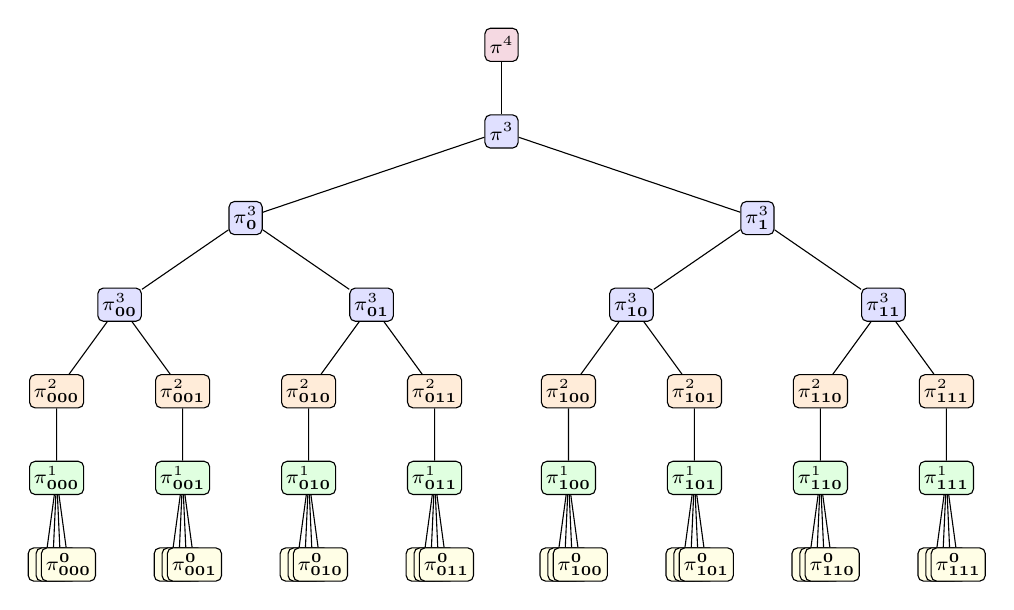
\begin{tikzpicture}[
		every node/.style={draw, rounded corners=2pt, minimum width=1.2em, minimum height=1.2em, inner sep=1.5pt, font=\scriptsize},
		embed/.style={fill=purple!15},
		combine/.style={fill=blue!12},
		convert/.style={fill=orange!15},
		riscv/.style={fill=green!12},
    base/.style={fill=yellow!10},
		level 1/.style={sibling distance=130mm},
		level 2/.style={sibling distance=65mm},
		level 3/.style={sibling distance=32mm},
		level 4/.style={sibling distance=16mm},
		level 5/.style={sibling distance=4mm},
		level 6/.style={sibling distance=1mm},
		level distance=11mm,
		edge from parent/.style={draw, thin},
		]
		\node [embed] {$\pi^{4}$}
		child { node [combine] {$\pi^{3}$}
			child {
				node [combine] {$\pi^{3}_{\bf 0}$}
				child {
					node [combine] {$\pi^{3}_{\bf 00}$}
					child { node [convert] {$\pi^{2}_{\bf 000}$}
						child { node [riscv] {$\pi^{1}_{\bf 000}$}
							child { node [base] {} }
							child { node [base] {} }
							child { node [base] {} }
							child { node [base] {$\pi^{\mathbf{0}}_{\bf 000}$} }
						}
					}
					child { node [convert] {$\pi^{2}_{\bf 001}$}
						child { node [riscv] {$\pi^{1}_{\bf 001}$}
							child { node [base] {} }
							child { node [base] {} }
							child { node [base] {} }
							child { node [base] {$\pi^{\mathbf{0}}_{\bf 001}$} }
						}
					}
				}
				child {
					node [combine] {$\pi^{3}_{\bf 01}$}
					child { node [convert] {$\pi^{2}_{\bf 010}$}
						child { node [riscv] {$\pi^{1}_{\bf 010}$}
							child { node [base] {} }
							child { node [base] {} }
							child { node [base] {} }
							child { node [base] {$\pi^{\mathbf{0}}_{\bf 010}$} }
						}
					}
					child { node [convert] {$\pi^{2}_{\bf 011}$}
						child { node [riscv] {$\pi^{1}_{\bf 011}$}
							child { node [base] {} }
							child { node [base] {} }
							child { node [base] {} }
							child { node [base] {$\pi^{\mathbf{0}}_{\bf 011}$} }
						}
					}
				}
			}
			child {
				node [combine] {$\pi^{3}_{\bf 1}$}
				child {
					node [combine] {$\pi^{3}_{\bf 10}$}
					child { node [convert] {$\pi^{2}_{\bf 100}$}
						child { node [riscv] {$\pi^{1}_{\bf 100}$}
							child { node [base] {} }
							child { node [base] {} }
							child { node [base] {} }
							child { node [base] {$\pi^{\mathbf{0}}_{\bf 100}$} }
						}
					}
					child { node [convert] {$\pi^{2}_{\bf 101}$}
						child { node [riscv] {$\pi^{1}_{\bf 101}$}
							child { node [base] {} }
							child { node [base] {} }
							child { node [base] {} }
							child { node [base] {$\pi^{\mathbf{0}}_{\bf 101}$} }
						}
					}
				}
				child {
					node [combine] {$\pi^{3}_{\bf 11}$}
					child { node [convert] {$\pi^{2}_{\bf 110}$}
						child { node [riscv] {$\pi^{1}_{\bf 110}$}
							child { node [base] {} }
							child { node [base] {} }
							child { node [base] {} }
							child { node [base] {$\pi^{\mathbf{0}}_{\bf 110}$} }
						}
					}
					child { node [convert] {$\pi^{2}_{\bf 111}$}
						child { node [riscv] {$\pi^{1}_{\bf 111}$}
							child { node [base] {} }
							child { node [base] {} }
							child { node [base] {} }
							child { node [base] {$\pi^{\mathbf{0}}_{\bf 111}$} }
						}
					}
				}
			}
		};
	\end{tikzpicture}
	\caption{\label{fig:topo} Recursion topology. Colors: \colorbox{yellow!10}{\texttt{inner}}, \colorbox{green!12}{\texttt{segment}}, \colorbox{orange!15}{\texttt{convert}}, \colorbox{blue!12}{\texttt{combine}}, \colorbox{purple!15}{\texttt{embed}}.}
\end{figure}

\subsection{\texttt{inner} circuits}

To optimize the proof size and prover time,
we introduce inner segment circuits that prove
the correctness of the segment trace, of precompiles,
and of range checks separately. As those
circuits share the same bus, we commit to the latter
to make the relations succinct.
These circuits are then recursively
combined  to prove the correctness of the full segment.

The first relation $\relation_{0,\step}$ chains
$N_{\text{seg}}$ consecutive valid steps
from $\hat{S}_{in}$ to $\hat{S}_{out}$,
with the bus committed in the public input.
The remaining three relations each assert correctness of
all entries of a given type in the bus
(Keccak, Poseidon, or range checks respectively),
again with the bus committed\footnote{Without loss
of generality we assume that the same commitment scheme is used for the bus.} in the public input.
\begin{equation}\label{eq:rel-inner-step}
  \scalebox{0.90}{$\displaystyle
    \relation_{0,\step} =\left(
    \left(\begin{array}{l}
      (\hat{S}_{in},\hat{S}_{out}, C_{\hat{\mathcal{B}}} );\;\\
      (\widehat{\BBB},\{\hat{S}_i\}_{1\leq i \leq {N_{\text{seg}}}+1},
      \{\pi^{\mathsf{mem}}_i\}_{1\leq i\leq N_{\text{seg}}})
    \end{array}\right)\;\Bigg|\quad
    \begin{array}{c}
      \hat{S}_1 = \hat{S}_{in}\\
      \hat{S}_{N_{\text{seg}}+1} = \hat{S}_{out}\\
      \bigwedge_{i=1}^{N_{\text{seg}}} \widehat{\pred{}}_{step,bus} (\hat{S}_i,\hat{S}_{i+1},\widehat{\BBB},\pi^{\mathsf{mem}}_i)=\mathrm{TRUE}\\
      C_{\hat{\mathcal{B}}} = \Com_{\mathsf{bus}}(\widehat{\BBB})
    \end{array}
   \right)
  $}
\end{equation}
where $\pi^{\mathsf{mem}}_i$ is the memory-opening witness for step~$i$: for a read step it is the Merkle authentication path $\pi$ required by $\widehat{\pred{}}_{\rea}$~\eqref{eq:op-mem-comm-read}; for a write step it is the pair $\pi^{\mathsf{mem}}_i = (\pi_{\writ}, v_{\mathsf{old}})$ required by $\widehat{\pred{}}_{\writ}$~\eqref{eq:op-mem-comm-write}; for all other steps it is unused.
The program code $\code$ is hard-wired into the \texttt{inner-step} circuit --- it appears in the fetch conjunct $\code[\pc_1]=op$ of each operation predicate via~\eqref{eq:phiop} --- so the \texttt{inner-step} verification key binds the proof to the fixed program.
\begin{equation}\label{eq:rel-inner-keccak}
  \relation_{0,\keccak} =\left(
   \left( C_{\hat{\mathcal{B}}} ;\;
  \widehat{\BBB} \right)\;\Bigg|\quad
  \begin{array}{c}
    \widehat{\pred{}}_{\keccak}(\widehat{\BBB})=\mathrm{TRUE}\\
    C_{\hat{\mathcal{B}}} = \Com_{\mathsf{bus}}(\widehat{\BBB})
  \end{array}
 \right)
\end{equation}
\begin{equation}\label{eq:rel-inner-poseidon}
  \relation_{0,\poseidon} =\left(
   \left( C_{\hat{\mathcal{B}}} ;\;
  \widehat{\BBB} \right)\;\Bigg|\quad
  \begin{array}{c}
    \widehat{\pred{}}_{\poseidon}(\widehat{\BBB})=\mathrm{TRUE}\\
    C_{\hat{\mathcal{B}}} = \Com_{\mathsf{bus}}(\widehat{\BBB})
  \end{array}
 \right)
\end{equation}
\begin{equation}\label{eq:rel-inner-range}
  \relation_{0,\range} =\left(
   \left( C_{\hat{\mathcal{B}}} ;\;
  \widehat{\BBB} \right)\;\Bigg|\quad
  \begin{array}{c}
    \widehat{\pred{}}_{\range}(\widehat{\BBB})=\mathrm{TRUE}\\
    C_{\hat{\mathcal{B}}} = \Com_{\mathsf{bus}}(\widehat{\BBB})
  \end{array}
 \right)
\end{equation}

The circuits are called, respectively,
\texttt{inner-step}, \texttt{inner-keccak}, \texttt{inner-poseidon}, and \texttt{inner-range}.
\begin{instruction}
Note that our writeup is a bit informal here, as we never formally defined $\Com$. Teams should do that, as the security analysis later will require a specific binding notion of $\Com$.
\end{instruction}

\subsection{ \texttt{segment} circuit}

The \texttt{segment} circuit recursively verifies the four inner proofs,
tying them together via a shared bus commitment $C_{\hat{\mathcal{B}}}$.
Let $\Pi_{0,j}=(\Pi_{0,j}.\mathsf{Prove}, \Pi_{0,j}.\mathsf{Verify})$
be the SNARK for $\relation_{0,j}$, where $j\in\{\step,\keccak,\poseidon,\range\}$.

\[
  \scalebox{0.90}{$\displaystyle
  \relation_1=\left\lbrace\begin{array}{c|c} (\hat{S}_{in},
   \hat{S}_{out});(C_{\hat{\mathcal{B}}},\pi_\step,\pi_\keccak,\pi_\poseidon,\pi_\range) &
    \begin{array}{c}
   \Pi_{0,\step}.\mathsf{Verify}((\hat{S}_{in},\, \hat{S}_{out},\, C_{\hat{\mathcal{B}}}), \pi_\step)=1\\
    \Pi_{0,\keccak}.\mathsf{Verify}( C_{\hat{\mathcal{B}}}, \pi_\keccak)=1\\
    \Pi_{0,\poseidon}.\mathsf{Verify}( C_{\hat{\mathcal{B}}}, \pi_\poseidon)=1\\
    \Pi_{0,\range}.\mathsf{Verify}( C_{\hat{\mathcal{B}}}, \pi_\range)=1
    \end{array}
  \end{array}\right\rbrace
  $}
\]


\subsection{\texttt{convert} circuit}

The \texttt{convert} circuit is a 1-to-1 recursion circuit that consumes a proof of $\relation_1$ and verifies it.  Its public
inputs are the boundary states and the segment size; its witness is the proof $\pi_1$. To formally define the relation,
let $\Pi_1=(\Pi_1.\mathsf{Prove}, \Pi_1.\mathsf{Verify})$ be the SNARK proving protocol for relation $\relation_1$.

$$\relation_2=\left\lbrace\begin{array}{c|c}
	((\hat{S}_0,\, \hat{S}_N,\, {N_{\text{seg}}});\; \pi_1) &
	\Pi_1.\mathsf{Verify}((\hat{S}_0,\, \hat{S}_N), \pi_1)=1
\end{array}\right\rbrace$$
Note that triples for which the last component is not ${N_{\text{seg}}}$ are never in $\relation_2$.

\subsection{\texttt{combine} circuit}

The \texttt{combine} circuit is a recursive 2-to-1 circuit that verifies two child proofs, each of which may be either a \texttt{convert} proof or another \texttt{combine} proof.
It checks three things:
\begin{itemize}
\item Each child proof is valid under $\Pi_2.\mathsf{Verify}$ if the child covers exactly one segment ($N_{child}=N_{\seg}$), or under $\Pi_3.\mathsf{Verify}$ if it covers at least two ($N_{child}\ge 2N_{\seg}$), where $\Pi_i=(\Pi_i.\mathsf{Prove}, \Pi_i.\mathsf{Verify})$ is the SNARK proving protocol for relation $\relation_i$.
\item The step counts satisfy $N_L + N_R = N$, with $N_L \geq N_{\seg}$, $N_R \geq N_{\seg}$, and both $N_L$, $N_R$ divisible by $N_{\seg}$, to ensure well-founded recursion and uniform segment structure.
\item State continuity: the witness $\hat{S}_N^L$ serves as both the final state of the left proof and the initial state of the right proof.
\end{itemize}
Since \texttt{combine} is self-recursive, repeated binary application naturally reduces any number of segment proofs into a single proof $\pi_3$ for the full execution.

For brevity, we write $\Vfy_i(\mathsf{x},\pi):=\Pi_i.\mathsf{Verify}(\mathsf{x},\pi)$.
\begin{equation}\label{eq:rel-combine-typed}
  \scalebox{0.85}{$\displaystyle
  \relation_3=\left\lbrace\begin{array}{c|c}
   ((\hat{S}_0^L,\, \hat{S}_N^R,\, N);\; (\pi^L,\, \pi^R,\, \hat{S}_N^L, N_L, N_R)) &
    \begin{array}{c}
   \bigl(N_L = N_{\seg} \wedge \Vfy_2((\hat{S}_0^L, \hat{S}_N^L, N_L),\, \pi^L)=1\bigr) \\
   {}\lor \bigl(N_L \geq 2N_{\seg} \wedge \Vfy_3((\hat{S}_0^L, \hat{S}_N^L, N_L),\, \pi^L)=1\bigr) \\
   \bigl(N_R = N_{\seg} \wedge \Vfy_2((\hat{S}_N^L, \hat{S}_N^R, N_R),\, \pi^R)=1\bigr) \\
   {}\lor \bigl(N_R \geq 2N_{\seg} \wedge \Vfy_3((\hat{S}_N^L, \hat{S}_N^R, N_R),\, \pi^R)=1\bigr) \\
   N_L + N_R = N \\
   N_{\seg} \mid N_L,\; N_{\seg} \mid N_R
    \end{array}
  \end{array}\right\rbrace
  $}
\end{equation}

where $\hat{S}_0^L$ and $\hat{S}_N^R$ are the public boundary states of the combined execution,
$\pi^L$ and $\pi^R$ are the two child proofs (each either a \texttt{convert} or \texttt{combine} proof), and $\hat{S}_N^L$ is the intermediate boundary state provided as witness.
The step count decides the child's type: a child covering exactly one segment
must carry a \texttt{convert} proof, a larger child a \texttt{combine} proof.
This typing is what entitles the extraction argument
(Lemma~\ref{lem:combine}) to treat every $\Vfy_2$-verified child as a
single-segment leaf: \emph{verification} of a proof for a statement outside a
relation's support is not excluded by knowledge soundness, so without the
typing the extractor could meet a verifying \texttt{convert} proof at a step
count it cannot use.  Completeness is unaffected --- an honest prover's
children have exactly these types.  (The bounds $N_L,N_R\ge N_{\seg}$ of the
untyped formulation are implied by the typing.)

\subsection{\texttt{embed} circuit}

The \texttt{embed} circuit produces the final proof, asserting correctness of the entire program execution
with public initial and final states. It assumes that
the total step count $T$ is known in advance to the verifier.
We fix $T$ as a publicly known system parameter satisfying $T \geq 2N_{\seg}$ and $N_{\seg} \mid T$
throughout, with $T \leq \mathsf{poly}(\lambda)$; these are standing assumptions on the system parameters and are not constraints
enforced by the circuit itself. The lower bound $T \geq 2N_{\seg}$ ensures that every execution
has at least two segments and hence admits a well-formed \texttt{combine} proof tree: a
single-segment execution ($T = N_{\seg}$) cannot be proven, because $\relation_3$ requires
$N_L + N_R = N$ with $N_L, N_R \geq N_{\seg}$, i.e.\ $N \geq 2N_{\seg}$.
Let $\Pi_3=(\Pi_3.\mathsf{Prove}, \Pi_3.\mathsf{Verify})$ be the SNARK proving protocol for relation $\relation_3$.

$$\relation_4=\left\lbrace\begin{array}{c|c}
	((\hat{S}_0,\, \hat{S}_T);\; \pi_3) &
	\Pi_3.\mathsf{Verify}((\hat{S}_0,\, \hat{S}_T,\,T),\, \pi_3)=1
\end{array}\right\rbrace$$

where $\hat{S}_0$ and $\hat{S}_T$ are the initial and final states of the entire program execution.

\begin{remark}[Divisibility requirement on $T$]
Since $\relation_3$ requires both child step counts to be divisible by $N_{\seg}$, every well-formed
\texttt{combine} proof tree has a total step count $N$ that is a multiple of $N_{\seg}$.
Consequently, the total step count $T$ passed to the \texttt{embed} circuit must satisfy
$N_{\seg} \mid T$.  The verifier checks this divisibility before invoking
$\Pi_3.\mathsf{Verify}$; proofs for step counts not divisible by $N_{\seg}$ are rejected outright.
\end{remark}

\begin{instruction}
  Teams should explain how the relations are proven using AIR / IOPs / poly-IOPs and the BCS transform. That is, teams should provide a direct reduction
from proving a relation to a low-degree test with
  FRI or another protocol. The reductions should contain links to the circuits submitted to soundcalc.
  The purpose of the section is to make explicit how the relations from the previous section are proven.
\end{instruction}

%----------------------------------------------------------------------

\section{Security}\label{sec:security}
%----------------------------------------------------------------------

We prove that the zkVM construction is \emph{correct-trace extractable}: any
adversary that produces a convincing final proof can be used to extract an
explicit, valid execution trace.  The proof proceeds by descending the recursion
tree layer by layer, reducing everything ultimately to the knowledge soundness
of the inner-circuit SNARKs, the binding properties
of the memory commitment scheme $\Com_{\mathsf{mem}}$, and the collision-resistance of $\Com_{\mathsf{bus}}$.

\begin{remark}[Idealized proof model]\label{rem:idealized}
Our proof is idealized/heuristic in two respects.

First, Definition~\ref{def:extractable} below postulates a straight-line
extractor that runs in essentially the time of the adversary, with only
additive $\mathsf{poly}(\lambda)$ overhead. Because our SNARKs are hash-based,
the natural model is the random oracle model (ROM), in which such
straight-line extractors do exist. The subtlety lies in the recursion:
composing straight-line extraction across the layers of the proof tree (as in
proof-carrying data, PCD) requires each SNARK to remain knowledge-sound
\emph{relative to the same random oracle}, i.e.\ to be a \emph{relativized}
argument system, and such relativized SNARKs provably do not exist in general
\cite{EPRINT:relativized}. Our analysis idealizes over this obstruction: we assume that straight-line extraction composes across the
recursion, effectively putting the non-existence of relativized SNARKs under
the rug.

Second, while the analysis does produce explicit advantage bounds and reduction
running times (Theorem~\ref{thm:main}), the idealization above means these
should not be read as a concrete security level: they are meaningful as a
statement about the reduction structure --- the recursion topology is sound and
the circuit relations compose consistently --- but a concrete security claim
would require replacing the idealized straight-line extraction assumption with
an analysis of the actual instantiation.
\end{remark}

%----------------------------------------------------------------------
\subsection{Definitions}\label{sec:security:defs}
%----------------------------------------------------------------------

We work with knowledge-sound argument systems admitting straight-line
extraction.  Let $\lambda$ denote the security parameter;
``PPT'' means probabilistic polynomial time in $\lambda$.

\begin{definition}[Knowledge-soundness]\label{def:extractable}
A non-interactive argument system $\Pi=(\mathsf{Prove},\mathsf{Verify})$ for
relation $\mathcal{R}$ is \emph{knowledge-sound} if there exists a PPT
algorithm $\mathcal{E}$ (the \emph{extractor}) such that for every PPT
adversary $\mathcal{A}$:
\begin{equation}\label{eq:extractable}
  \mathsf{Adv}^{\mathsf{ks}}_{\Pi}(\mathcal{A}) \;:=\;
  \Pr\!\Bigl[
    (x,\pi)\leftarrow\mathcal{A}(1^\lambda);\; w\leftarrow\mathcal{E}(x,\pi)
    \;:\; \Pi.\mathsf{Verify}(x,\pi)=1 \;\wedge\; (x;\,w)\notin\mathcal{R}
  \Bigr] \leq \mathsf{negl}(\lambda).
\end{equation}

We assume that the running time of $\mathcal{E}(x,\pi)$ is at most
$\mathsf{Time}(\mathcal{A}(1^\lambda)) + \mathsf{poly}(\lambda)$ for every
adversary $\mathcal{A}$ and every $(x,\pi)$ in the support of $\mathcal{A}$'s
output, i.e.\ the
extractor incurs only an additive polynomial overhead over a single evaluation of
$\mathcal{A}$ on the given proof.
We call $\mathsf{Adv}^{\mathsf{ks}}_{\Pi}(\mathcal{A})$ the knowledge-soundness
error of $\mathcal{A}$ against $\Pi$.
\end{definition}

\begin{remark}[Straight-line extraction]
The extractor $\mathcal{E}$ above is straight-line: it takes only the
statement $x$ and the proof $\pi$ as input and does not rewind $\mathcal{A}$. This can actually not be achieved if $\pi$ is succinct, but this is part of our (over-)idealization, see Remark~\ref{rem:idealized} above. Namely, Definition~\ref{def:extractable} is
an idealized requirement that cannot be satisfied by any standard construction
in the plain model (see Remark~\ref{rem:idealized}).  It serves as a
\emph{proxy}: we state it formally so that the reduction structure is
explicit, with the understanding that concrete instantiations will replace it
with ROM-based extractability at the cost of the overhead
discussed in Remark~\ref{rem:idealized}.
\end{remark}

\begin{instruction}
  In the following, we omit commitment keys for simplicity of exposition. Teams should add appropriate definitions and adaptations if they rely on commitment keys.
\end{instruction}

\begin{instruction}
  We also leave out completeness definitions, as the document should just illustrate the structure of a potential soundness proof. Teams should add completeness arguments as well.
\end{instruction}

\begin{definition}[Position-binding and update-binding vector commitment]\label{def:binding}
A vector commitment scheme
$\Com=(\mathsf{Commit},\mathsf{Open},\mathsf{Verify})$
satisfies the two independent properties below --- \emph{position-binding} and
\emph{update-binding} --- which a scheme may have separately or together.
\begin{enumerate}
  \item \textbf{Position-binding.} For every PPT adversary $\mathcal{A}$, the following is negligible:
\[
  \mathsf{Adv}^{\mathsf{pos}}_{\Com}(\mathcal{A}) \;:=\;
  \Pr\!\left[\begin{array}{l}
    (C,i,v,\pi,v',\pi')\leftarrow\mathcal{A}(1^\lambda) \;:\; \\[4pt]
    \mathsf{Verify}(C,i,v,\pi)=1 \;\wedge\;
    \mathsf{Verify}(C,i,v',\pi')=1 \;\wedge\; v\neq v'
  \end{array}\right].
\]
  \item \textbf{Update binding.} For every PPT adversary $\mathcal{A}$, the
    following is negligible, where $C:=\mathsf{Commit}(\vec{m})$:
\[
  \mathsf{Adv}^{\mathsf{upd}}_{\Com}(\mathcal{A}) \;:=\;
  \Pr\!\left[\begin{array}{l}
    (\vec{m}, \addr, x, C', \pi) \leftarrow \mathcal{A}(1^\lambda) \;:\; \\[4pt]
    \mathsf{Verify}(C,\addr,\vec{m}[\addr],\pi)=1 \;\wedge\;
    \mathsf{Verify}(C',\addr,x,\pi)=1 \\[4pt]
    {}\wedge\; C' \neq \mathsf{Commit}(\vec{m}[\addr\mapsto x])
  \end{array}\right].
\]
In other words, a single opening proof $\pi$ that opens an honest commitment
$C=\mathsf{Commit}(\vec{m})$ at position $\addr$ and also opens $C'$ at $\addr$
to $x$ forces $C'$ to be the honest commitment of the updated vector
$\vec{m}[\addr\mapsto x]$. In particular $C'$ is then itself a well-formed
commitment --- an actual output of $\mathsf{Commit}$ --- and not merely a value
that verifies against some proofs.
\end{enumerate}
\end{definition}
\begin{remark}[Merkle trees and update binding]
Standard Merkle tree commitments satisfy both position-binding and update
binding under collision-resistance of the underlying hash function.  The
position-binding property is immediate.  For update binding, a Merkle
authentication path $\pi$ for position $\addr$ consists of the sibling hashes
along the root-to-leaf path; since $C=\mathsf{Commit}(\vec{m})$ is honest, those
siblings must --- except for a hash collision --- be the honest siblings of
$\vec{m}$, so recomputing the root with the new leaf $x$ yields exactly
$\mathsf{Commit}(\vec{m}[\addr\mapsto x])$, and no other value of $C'$ can pass.
We leave out a formal proof for now.
\end{remark}

\begin{definition}[Collision-resistant bus commitment]\label{def:bus-cr}
A bus commitment scheme $\Com_{\mathsf{bus}}$ is \emph{collision-resistant} if for every PPT adversary $\mathcal{A}$, the following is negligible:
\[
\mathsf{Adv}^{\mathsf{cr}}_{\Com_{\mathsf{bus}}}(\mathcal{A}):= \Pr\!\left[\begin{array}{l}
    (\widehat{\BBB},\widehat{\BBB}') \leftarrow \mathcal{A}(1^\lambda) \;:\; \\[4pt]
    \widehat{\BBB}\neq\widehat{\BBB}' \;\wedge\;
    \Com_{\mathsf{bus}}(\widehat{\BBB})=\Com_{\mathsf{bus}}(\widehat{\BBB}')
  \end{array}\right].
\]
\end{definition}



\begin{definition}[zkVM system]\label{def:zkvm}
A \emph{zkVM system} is a tuple
\[
  \mathsf{zkVM} = \bigl(
    \{\varphi_{\op}\}_{\op},\;
    \Com_{\mathsf{bus}},\;
    \Com_{\mathsf{mem}},\;
    \Pi_0,\, \Pi_1,\, \Pi_2,\, \Pi_3,\, \Pi_4
  \bigr)
\]
consisting of the following components.
\begin{enumerate}
  \item \textbf{Step predicates.}  For each operation $\op$ (including
    $\step$, $\rea$, $\writ$, $\keccak$, $\poseidon$, $\range$), a
    predicate $\varphi_{\op}$ over VM states, expressible as a system of
    polynomial constraints over the field (as defined in
    Section~\ref{sec:proof-arch}).

  \item \textbf{Bus commitment scheme.}
    $\Com_{\mathsf{bus}}$ is a collision-resistant
    bus commitment scheme (Definition~\ref{def:bus-cr}) used to commit to the shared bus
    $\mathcal{B}$ in the inner-circuit relations $\relation_{0,j}$.

  \item \textbf{Memory commitment scheme.}
    $\Com_{\mathsf{mem}} = (\mathsf{Commit}, \mathsf{Open}, \mathsf{Verify})$,
    a position-binding and update-binding vector commitment scheme
    (Definition~\ref{def:binding}) used to represent the memory component
    of each committed VM state $\hat{S}$.

  \item \textbf{SNARK hierarchy.}
    \begin{itemize}
      \item $\Pi_0 = \{\Pi_{0,j}\}_{j \in \{\step,\keccak,\poseidon,\range\}}$:
        the four \emph{inner-circuit} SNARKs for relations
        $$\relation_{0,\step},\, \relation_{0,\keccak},\,
         \relation_{0,\poseidon},\, \relation_{0,\range},$$ respectively.
      \item $\Pi_1$: the \texttt{segment} SNARK for relation $\relation_1$
        (verifies the four inner proofs).
      \item $\Pi_2$: the \texttt{convert} SNARK for relation $\relation_2$
        (1-to-1 normalization).
      \item $\Pi_3$: the \texttt{combine} SNARK for relation $\relation_3$
        (2-to-1 recursive merging).
      \item $\Pi_4$: the \texttt{embed} SNARK for relation $\relation_4$
        (final proof).
    \end{itemize}
    Each $\Pi_i = (\Pi_i.\mathsf{Prove}, \Pi_i.\mathsf{Verify})$ is a
    non-interactive argument system for the respective relation.
\end{enumerate}
\end{definition}

\begin{definition}[Correct-execution relation]\label{def:relation-star}
Fix a program code $\code$ and a step count $T$ satisfying $N_{\seg}\mid T$,
$T\ge 2N_{\seg}$, and $T\le\mathsf{poly}(\lambda)$ (system parameters, as in the
\texttt{embed} circuit of Section~\ref{sec:proof-arch}); neither $\code$ nor $T$
is chosen by the adversary.

The \emph{correct-execution relation} $\relation^*=\relation^*_{\code,T}$ has as
statements boundary pairs $(S_0,S_T)$ of full-memory VM states
$S=(\pc,\regs,\mem)$, and as witnesses candidate full-memory traces
$(S_0',\ldots,S_T')$:
\begin{equation}\label{eq:relation-star}
  \relation^* \;=\; \left\{\,\bigl((S_0,S_T);\;(S_0',\ldots,S_T')\bigr)\;\middle|\;
    S_0'=S_0 \;\wedge\; S_T'=S_T \;\wedge\;
    \forall i\in[T]:\varphi_{\step}(S_{i-1}',S_i')=\mathrm{TRUE}
  \right\},
\end{equation}
where $\varphi_{\step}$ is the step predicate of Section~\ref{sec:proof-arch}
(the disjunction over all operation predicates $\varphi_{\op}$).
\end{definition}

\begin{definition}[Final argument system]\label{def:final-as}
The \emph{final argument system} of $\mathsf{zkVM}$ is the non-interactive
argument system $\Pi^*=(\Pi^*.\mathsf{Prove},\Pi^*.\mathsf{Verify})$ for the
correct-execution relation $\relation^*$ (Definition~\ref{def:relation-star})
whose proofs are the final \texttt{embed} proofs $\pi^4$ and whose verification
algorithm, on statement $(S_0,S_T)$ and proof $\pi^4$, proceeds as follows:
\begin{enumerate}
  \item set
    $$\hat{S}_0 := (\pc_0,\regs_0,\mathsf{Commit}(\mem_0)),\quad
    \hat{S}_T := (\pc_T,\regs_T,\mathsf{Commit}(\mem_T));$$
  \item output $\Pi_4.\mathsf{Verify}((\hat{S}_0,\hat{S}_T),\pi^4)$,
\end{enumerate}
where $\mathsf{Commit}$ is that of $\Com_{\mathsf{mem}}$.  Its prover
$\Pi^*.\mathsf{Prove}$ is the honest proving pipeline of
Section~\ref{sec:proof-arch} instantiated at $(\code,T)$; it plays no role in
what follows.\footnote{Observe that the definition of knowledge soundness just
depends on a verification algorithm and not on the associated prover.}
\end{definition}

\begin{definition}[Correct-trace extractability]\label{def:cte}
The zkVM $\mathsf{zkVM}$ is \emph{correct-trace extractable} if its final
argument system $\Pi^*$ (Definition~\ref{def:final-as}) is knowledge-sound for
the correct-execution relation $\relation^*$ (Definition~\ref{def:relation-star})
in the sense of Definition~\ref{def:extractable}.  We write
\[
  \mathsf{Adv}^{\mathsf{cte}}_{\mathsf{zkVM}}(\mathcal{A})
  \;:=\;\mathsf{Adv}^{\mathsf{ks}}_{\Pi^*}(\mathcal{A})
\]
for the \emph{CTE advantage} of a PPT adversary $\mathcal{A}$, and
$\mathcal{E}_{\mathsf{zkVM}}$ for the extractor whose existence is asserted; the
additive running-time convention of Definition~\ref{def:extractable} applies to
it unchanged.
\end{definition}

\begin{remark}[Unrolling Definition~\ref{def:cte}]\label{rem:cte-experiment}
Written out, Definition~\ref{def:cte} says that there is a PPT extractor
$\mathcal{E}_{\mathsf{zkVM}}$ such that for every PPT adversary $\mathcal{A}$ the
experiment
\[
  \mathsf{Exp}_{\mathsf{zkVM},\mathcal{E}_{\mathsf{zkVM}},\mathcal{A}}^{\mathsf{cte}}(\lambda)
\]
below returns $1$ with at most negligible probability.
\begin{enumerate}
  \item \textbf{Adversary.} $\mathcal{A}(1^\lambda)$ outputs a statement
    $(S_0,S_T)$ --- an initial state $S_0=(\pc_0,\regs_0,\mem_0)$ and a final
    state $S_T=(\pc_T,\regs_T,\mem_T)$ --- together with a proof $\pi^4$; the
    program code $\code$ and step count $T$ are fixed system parameters.
  \item \textbf{Verification.} If $\Pi^*.\mathsf{Verify}((S_0,S_T),\pi^4)=0$
    (Definition~\ref{def:final-as}), return $0$.
  \item \textbf{Extraction.} Run $\mathcal{E}_{\mathsf{zkVM}}(S_0,S_T,\pi^4)$ to
    obtain full-memory VM states $S_0',S_1',\ldots,S_T'$, where
    $S_i'=(\pc_i',\regs_i',\mem_i')$.
  \item \textbf{Winning condition.} Return $1$ (adversary wins) if and only if
    $\bigl((S_0,S_T);(S_0',\ldots,S_T')\bigr)\notin\relation^*$, i.e.\ if any of
    the following hold:
    \begin{itemize}
      \item $\pc_0' \neq \pc_0$, $\regs_0' \neq \regs_0$, or
        $\mem_0' \neq \mem_0$; or
      \item $\pc_T' \neq \pc_T$, $\regs_T' \neq \regs_T$, or
        $\mem_T' \neq \mem_T$; or
      \item $\varphi_{\step}(S_i', S_{i+1}') \neq \mathrm{TRUE}$ for some
        $i \in \{0,\ldots,T-1\}$.
    \end{itemize}
\end{enumerate}
This is Definition~\ref{def:extractable} instantiated at $(\relation^*,\Pi^*)$
verbatim; in particular the boundary checks are not extra requirements bolted
onto the game, but precisely the two boundary conjuncts
of~\eqref{eq:relation-star}.  Note also that a statement of $\relation^*$
carries the full memory vectors $\mem_0,\mem_T$, so $\Pi^*.\mathsf{Verify}$ is
not succinct; succinctness is a property of $\Pi_4$ and is orthogonal to
correct-trace extractability.
\end{remark}

%----------------------------------------------------------------------
\subsection{Memory extractability}\label{sec:security:bus}
%----------------------------------------------------------------------
The inner circuits operate on committed-memory states $\hat{S}$ and a bus
$\widehat{\BBB}$, whereas the correct-execution relation
$\relation^*$~\eqref{eq:relation-star} requires a valid
execution trace in terms of full-memory states $S$ with \emph{explicitly
reconstructed} memory vectors $\mem_k$.  The following proposition bridges
this gap and shows that, once the commitment openings are embedded in the
SNARK witnesses, the bus-based predicate implies the bus-free predicate:
introducing a bus does not weaken the correctness guarantee.  In particular,
position-binding and update-binding of $\Com_{\mathsf{mem}}$ bound the
probability that the extracted full-memory trace deviates from the
committed-memory execution recorded by the SNARKs.

It does so in three respects: (i)~it eliminates the bus; (ii)~it lifts the
step predicate from committed-memory states to full-memory states whose
values at accessed addresses are uniquely determined by the position-binding
commitment openings embedded in the SNARK witness; and (iii)~it carries the
commitment invariant $\hat{S}.\mem=\mathsf{Commit}(\mem)$ forward by one step,
so that the invariant is a \emph{conclusion} of the proposition rather than a
side condition established elsewhere.  Concretely, it shows
that if the bus-parameterised step predicate $\widehat{\varphi}_{\step}$
holds (as guaranteed by Lemma~\ref{lem:segment}), then the bus-free,
full-memory predicate $\varphi_{\step}(S_1,S_2)$ holds for the states
$S_j := (\hat{S}_j.\pc,\hat{S}_j.\regs,\mem_j)$ formed with the reconstructed
memory vectors, and $\hat{S}_2.\mem=\mathsf{Commit}(\mem_2)$; the required
memory values are extracted from the commitment openings embedded in the
definitions of $\widehat{\varphi}_{\rea}$ and $\widehat{\varphi}_{\writ}$.
It is invoked once per step in Step~6 of the proof of
Theorem~\ref{thm:main}, where the two conclusions are used respectively as the
per-step guarantee required by the step conjunct
of~\eqref{eq:relation-star} and as the induction
hypothesis for the next step.

The second memory vector is not a free choice of the adversary: it is obtained
from the first by the deterministic \emph{memory reconstruction rule}
\begin{equation}\label{eq:mem-reconstruct}
  \mem_2 \;:=\;
  \begin{cases}
    \mem_1[\,\hat{S}_1.\regs[0]\mapsto\hat{S}_1.\regs[1]\,]
      & \text{if } \code[\hat{S}_1.\pc]=\writ,\\[2pt]
    \mem_1 & \text{otherwise,}
  \end{cases}
\end{equation}
which is exactly the rule the extractor of Theorem~\ref{thm:main} applies when
it reconstructs the full-memory trace.  Fixing $\mem_2$ this way is what makes
the commitment invariant provable rather than assumable: an adversary that
could choose $\mem_2$ freely subject to $\hat{S}_2.\mem=\mathsf{Commit}(\mem_2)$
would already have been handed the invariant as a hypothesis, and the
update-binding term in the bound below would do no work.

Throughout, we write
\[
  \widehat{\varphi}_{\step}(\hat{S}_i,\hat{S}_{i+1},\widehat{\BBB})
\]
as shorthand for the four-argument predicate~\eqref{eq:step-bus2} instantiated
with the memory-opening witness $\pi^{\mathsf{mem}}_i$ that is carried alongside
the states:
\[
  \widehat{\varphi}_{\step}(\hat{S}_i,\hat{S}_{i+1},\widehat{\BBB},\pi^{\mathsf{mem}}_i)=\mathrm{TRUE}.
\]
The shorthand is \emph{not} an existential quantification over
$\pi^{\mathsf{mem}}_i$: the witness is a fixed entry of the extracted
$\relation_{0,\step}$ witness vector.  Wherever the shorthand and an explicit
memory-opening witness both occur --- as in
Proposition~\ref{prop:memory-extractability}, whose second and fourth
hypotheses each refer to $\pi^{\mathsf{mem}}$ --- they denote the same object,
so the disjunct of $\widehat{\varphi}_{\step,\bus}$ that is satisfied is the one
evaluated on that witness.

\begin{proposition}[Memory extractability]
  \label{prop:memory-extractability}
For every PPT adversary $\mathcal{A}$ that outputs a tuple
$$(\hat{S}_1,\hat{S}_2,\mem_1,\widehat{\BBB},\pi^{\mathsf{mem}})$$
such that, defining $\mem_2$ by the reconstruction
rule~\eqref{eq:mem-reconstruct} and writing
$S_j:=(\hat{S}_j.\pc,\hat{S}_j.\regs,\mem_j)$, the following hold with
probability $\varepsilon$:
\begin{itemize}
  \item $\hat{S}_1.\mem = \mathsf{Commit}(\mem_1)$;
  \item $\widehat{\varphi}_{\step}(\hat{S}_1,\hat{S}_2,\widehat{\BBB})=\mathrm{TRUE}$;
  \item the step fails to transfer, i.e.\ the commitment invariant is not
    carried forward or the full-memory step predicate does not hold:
    \[
      \hat{S}_2.\mem \neq \mathsf{Commit}(\mem_2)
      \qquad\text{or}\qquad
      \varphi_{\step}(S_1,S_2)\neq\mathrm{TRUE};
    \]
  \item the memory-opening witness $\pi^{\mathsf{mem}}$ satisfies,
    depending on the operation type:
    \begin{itemize}
      \item \emph{Read}: $\pi^{\mathsf{mem}} = \pi$ with
        $\hat{S}_1.\mem=\hat{S}_2.\mem$ and
        $\mathsf{Verify}(\hat{S}_1.\mem,\hat{S}_1.\regs[0],\hat{S}_2.\regs[1],\pi)=1$;
      \item \emph{Write}: $\pi^{\mathsf{mem}} = (\pi_{\writ}, v_{\mathsf{old}})$ with
        \begin{align*}
        &\mathsf{Verify}(\hat{S}_1.\mem,\hat{S}_1.\regs[0],v_{\mathsf{old}},\pi_{\writ})=1,\\
        &\mathsf{Verify}(\hat{S}_2.\mem,\hat{S}_1.\regs[0],\hat{S}_1.\regs[1],\pi_{\writ})=1;
        \end{align*}
      \item \emph{Other}: no condition is imposed on $\pi^{\mathsf{mem}}$;
    \end{itemize}
\end{itemize}
there exist PPT reduction adversaries $\mathcal{D}^{\mathsf{pos}}$ and
$\mathcal{D}^{\mathsf{upd}}$, each constructed from $\mathcal{A}$ and running
in time $\mathsf{Time}(\mathcal{A})+\mathsf{poly}(\lambda)$, such that
\[
  \varepsilon \leq\;
  \mathsf{Adv}^{\mathsf{pos}}_{\Com_{\mathsf{mem}}}(\mathcal{D}^{\mathsf{pos}})
  + \mathsf{Adv}^{\mathsf{upd}}_{\Com_{\mathsf{mem}}}(\mathcal{D}^{\mathsf{upd}}).
\]
Equivalently: whenever the first, second and fourth hypotheses hold, both
$\hat{S}_2.\mem=\mathsf{Commit}(\mem_2)$ and
$\varphi_{\step}(S_1,S_2)=\mathrm{TRUE}$, except with probability at most
$\mathsf{Adv}^{\mathsf{pos}}_{\Com_{\mathsf{mem}}}(\mathcal{D}^{\mathsf{pos}})
+\mathsf{Adv}^{\mathsf{upd}}_{\Com_{\mathsf{mem}}}(\mathcal{D}^{\mathsf{upd}})$.
\end{proposition}

\begin{remark}[On the fourth hypothesis]\label{rem:mem-ext-hyp4}
Two points about the case distinction in the fourth hypothesis.

First, the \emph{Other} case is deliberately unconstrained.  The remaining
disjuncts of~\eqref{eq:step-bus2} never read $\pi^{\mathsf{mem}}$, so nothing in
the construction forces its value on a non-memory step, and the extractor of
Lemma~\ref{lem:segment} returns whatever the prover placed in that witness
field.  Demanding $\pi^{\mathsf{mem}}=\bot$ there would be a requirement the
zkVM does not enforce, and would make the proposition inapplicable to exactly
those steps; the proof never uses it.

Second, which of the three cases applies is determined by
$\op:=\code[\hat{S}_1.\pc]$ and is therefore not a free choice of
$\mathcal{A}$.  Every $\varphi'_{\op}$ carries the fetch conjunct
$\code[\pc_1]=\op$ of~\eqref{eq:phiop} --- for the two precompiles it is carried
by the chip predicate $\widehat{\varphi}_{\op}(\widehat{\BBB})$ rather than by
the bus-membership disjunct itself --- so under the second hypothesis at most
one disjunct of $\widehat{\varphi}_{\step,\bus}$ can be satisfied.  The
operation type is thus well defined, and the case split in the proof below is
the same case split as the one above.
\end{remark}

\begin{proof}
We define two bad events, each a violation of one binding property of
$\Com_{\mathsf{mem}}$, and bound each by a single reduction that runs
$\mathcal{A}$ once. We then show (Step~A) that off both events the assumption
$\widehat{\varphi}_{\step}(\hat{S}_1,\hat{S}_2,\widehat{\BBB})=\mathrm{TRUE}$
forces both $\hat{S}_2.\mem=\mathsf{Commit}(\mem_2)$ and
$\varphi_{\op}(S_1,S_2)=\mathrm{TRUE}$ for the operation $\op$ selected by
the satisfied disjunct, and hence $\varphi_{\step}(S_1,S_2)=\mathrm{TRUE}$ ---
contradicting the third winning condition. A union bound then gives the claim.

\paragraph{Bad events.}
Run $\mathcal{A}(1^\lambda)$ to obtain
$(\hat{S}_1,\hat{S}_2,\mem_1,\widehat{\BBB},\pi^{\mathsf{mem}})$ and set $\mem_2$
by~\eqref{eq:mem-reconstruct}. By the first hypothesis
$\hat{S}_1.\mem=\mathsf{Commit}(\mem_1)$, correctness of
$\Com_{\mathsf{mem}}$ makes the honest opening $\mathsf{Open}(\mem_1,p)$ verify
against $\hat{S}_1.\mem$ at every position $p$.

All memory vectors have the same length $n$, fixed by the system parameters,
and positions range over the index domain $[n]$.  Writing
$\addr:=\hat{S}_1.\regs[0]$ and $x:=\hat{S}_1.\regs[1]$, let
\[
  \mathcal{V}\;:=\;\{\,\mem_1,\;\mem_2\,\}
\]
be the \emph{candidate vectors}.  Both have length $n$ and are computable in
time $\mathsf{poly}(\lambda)$ from $\mathcal{A}$'s output --- $\mem_2$ because
the reconstruction rule~\eqref{eq:mem-reconstruct} is deterministic and
explicit --- so a reduction may open either of them honestly at any position.
Note that on a write step $\mem_2$ \emph{is} the updated vector
$\mem_1[\addr\mapsto x]$, so $\mathcal{V}$ already contains every vector the
argument below opens.  The well-formedness conjunct of $\varphi'_{\rea}$ and
$\varphi'_{\writ}$ guarantees $\addr\in[n]$ on the two memory operations, so
$\mem_1[\addr]$, $\mathsf{Open}(\mem_1,\addr)$ and $\mem_1[\addr\mapsto x]$ are
all well defined there.  Define:
\begin{itemize}
  \item $E_{\mathsf{pos}}$ (\emph{position-binding collision}): there are a root
    $R\in\{\hat{S}_1.\mem,\hat{S}_2.\mem\}$, a position $p$, and two accepting
    openings of $R$ at $p$ to distinct values, each either read from
    $\pi^{\mathsf{mem}}$ or computed as an honest opening $\mathsf{Open}(\vec{v},p)$
    of a candidate vector $\vec{v}\in\mathcal{V}$.
  \item $E_{\mathsf{upd}}$ (\emph{update-binding collision}):
    $\pi^{\mathsf{mem}}=(\pi_{\writ},v_{\mathsf{old}})$ is a write witness whose
    shared path $\pi_{\writ}$ opens the honest commitment $\hat{S}_1.\mem$ at
    $\addr:=\hat{S}_1.\regs[0]$ to $\mem_1[\addr]$ and opens $\hat{S}_2.\mem$ at
    $\addr$ to $x:=\hat{S}_1.\regs[1]$, yet
    $\hat{S}_2.\mem\neq\mathsf{Commit}(\mem_1[\addr\mapsto x])$.
\end{itemize}

\paragraph{The two reductions.}
$\mathcal{D}^{\mathsf{pos}}$ runs $\mathcal{A}(1^\lambda)$ once, then compares the
candidate vectors in $\mathcal{V}$ pairwise and against the values opened by
$\pi^{\mathsf{mem}}$; whenever
$E_{\mathsf{pos}}$ occurs it computes the corresponding honest openings and
outputs the two openings
$(R,p,v,\rho)$ and $(R,p,v',\rho')$ with $v\neq v'$ to the position-binding
challenger, breaking it. Hence
$\Pr[E_{\mathsf{pos}}]\le\mathsf{Adv}^{\mathsf{pos}}_{\Com_{\mathsf{mem}}}(\mathcal{D}^{\mathsf{pos}})$.
$\mathcal{D}^{\mathsf{upd}}$ runs $\mathcal{A}(1^\lambda)$ once; whenever
$E_{\mathsf{upd}}$ occurs it outputs
\[
  (\mem_1,\addr,x,\hat{S}_2.\mem,\pi_{\writ})
\]
to the update-binding challenger, breaking it: $\hat{S}_1.\mem=\mathsf{Commit}(\mem_1)$
is honest, the shared path $\pi_{\writ}$ opens it at $\addr$ to $\mem_1[\addr]$
and opens $\hat{S}_2.\mem$ at $\addr$ to $x$, yet
$\hat{S}_2.\mem\neq\mathsf{Commit}(\mem_1[\addr\mapsto x])$. Hence
$\Pr[E_{\mathsf{upd}}]\le\mathsf{Adv}^{\mathsf{upd}}_{\Com_{\mathsf{mem}}}(\mathcal{D}^{\mathsf{upd}})$.
Each reduction makes one run of $\mathcal{A}$, a linear scan of the candidate
vectors and a constant number of honest openings, so both run in time
$\mathsf{Time}(\mathcal{A})+\mathsf{poly}(\lambda)$ (note that $\mathcal{A}$
itself outputs $\mem_1$ and hence already runs in time $\Omega(n)$).

\paragraph{Step~A: off both events, the invariant and the step predicate transfer.}
\textit{Goal:} assuming $\neg E_{\mathsf{pos}}\wedge\neg E_{\mathsf{upd}}$,
\[
  \widehat{\varphi}_{\step}(\hat{S}_1,\hat{S}_2,\widehat{\BBB})=\mathrm{TRUE}
\]
implies $\hat{S}_2.\mem=\mathsf{Commit}(\mem_2)$ and
$\varphi_{\step}(S_1,S_2)=\mathrm{TRUE}$.  For the second conclusion we prove the
sharper statement that $\varphi_{\op}(S_1,S_2)=\mathrm{TRUE}$ for the operation
$\op$ whose disjunct of $\widehat{\varphi}_{\step,\bus}$ is satisfied; since
$\varphi_{\step}(S_1,S_2)$ is by definition the disjunction of the
$\varphi_{\op}(S_1,S_2)$ over all operations, the goal follows at once.
Every statement below is deterministic given
$\neg E_{\mathsf{pos}}\wedge\neg E_{\mathsf{upd}}$.
By Eq.~\eqref{eq:step-bus2}, the assumption expands as
\[
  \widehat{\varphi}_{\step}(\hat{S}_1,\hat{S}_2,\widehat{\BBB})
  \;=\;
  \widehat{\varphi}_{\step,\bus}(\hat{S}_1,\hat{S}_2,\widehat{\BBB})
  \;\wedge\;
  \widehat{\varphi}_{\keccak}(\widehat{\BBB})
  \;\wedge\;
  \widehat{\varphi}_{\poseidon}(\widehat{\BBB})
  \;\wedge\;
  \widehat{\varphi}_{\range}(\widehat{\BBB})
  \;=\;\mathrm{TRUE},
\]
so in particular
$\widehat{\varphi}_{\step,\bus}(\hat{S}_1,\hat{S}_2,\widehat{\BBB})=\mathrm{TRUE}$
and all chip predicates hold.

\smallskip
\noindent\emph{(No full-memory bus.)} The argument goes directly from the
committed, bus-parameterised predicate to the bus-free, full-memory predicate
$\varphi_{\step}(S_1,S_2)$; it never constructs a full-memory bus $\mathcal{B}$
and never invokes the bus-parameterised
form~\eqref{eq:step-expanded} of the step predicate.  This is deliberate, and
necessary: $\widehat{\BBB}$ is the bus of a whole segment
(Lemma~\ref{lem:segment}), so it carries range-check and precompile entries
belonging to \emph{other} steps, for which no memory vectors are extracted and
no full-memory states exist.  A predicate such as
$\varphi_{\keccak}(\mathcal{B})$, which quantifies over all entries of the bus,
therefore could not even be stated here, let alone established.  Instead each
bus-deferred obligation enters the case analysis on the committed side only, via
the chip predicates $\widehat{\varphi}_{\range}(\widehat{\BBB})$ and
$\widehat{\varphi}_{\op}(\widehat{\BBB})$ above, and is consumed at the single
bus entry belonging to this step.

\smallskip
\noindent\emph{(No commitment-injectivity argument.)} Because $\mem_2$ is
fixed by the reconstruction rule~\eqref{eq:mem-reconstruct} rather than chosen
by $\mathcal{A}$, the case analysis never has to infer an equality of vectors
from an equality of their commitments: each case obtains the memory component
of $\varphi_{\op}(S_1,S_2)$ directly from~\eqref{eq:mem-reconstruct}, and
obtains the invariant $\hat{S}_2.\mem=\mathsf{Commit}(\mem_2)$ either from the
commitment-equality conjunct of the disjunct (all cases but $\writ$) or from
update binding (the case $\writ$).  Position binding is used only to pin the
\emph{value} at the accessed address, at the single position $\addr$.
\begin{instruction}
  Here, and in some other places of the proofs, we implicitly used correctness of the vector commitment scheme, which we never explicitly defined. Team are expected to be less sloppy in this regard.
\end{instruction}

\smallskip

We case-split on the satisfied disjunct of $\widehat{\varphi}_{\step,\bus}$
(cf.~\eqref{eq:step-bus2}).  By Remark~\ref{rem:mem-ext-hyp4} the satisfied
disjunct is the one belonging to $\op=\code[\hat{S}_1.\pc]$, so the case
distinction below is the same one that drives the reconstruction
rule~\eqref{eq:mem-reconstruct}.

\smallskip
\noindent\emph{(Invariant, all cases but $\writ$.)} In the four non-write cases
$\op\neq\writ$, so~\eqref{eq:mem-reconstruct} sets $\mem_2:=\mem_1$, and the
satisfied disjunct asserts the commitment equality
$\hat{S}_1.\mem=\hat{S}_2.\mem$.  The invariant is then immediate,
\[
  \hat{S}_2.\mem=\hat{S}_1.\mem=\mathsf{Commit}(\mem_1)=\mathsf{Commit}(\mem_2),
\]
with no appeal to either binding property, and the memory conjunct
$\mem_2=\mem_1$ of $\varphi_{\op}$ holds by construction.  We record this once
and do not repeat it in the four cases below; only the write case, where the
commitment genuinely changes, needs update binding.

\smallskip
\begin{itemize}
\item \textbf{Non-memory arithmetic} ($\op_1,\ldots,\op_{10}$).
  The disjunct asserts
  $\widehat{\varphi}_{\op}(\hat{S}_1,\hat{S}_2)\wedge\hat{S}_1.\mem=\hat{S}_2.\mem$.
  The arithmetic part gives
  $\varphi'_{\op}(\hat{S}_1.\pc,\hat{S}_1.\regs,\hat{S}_2.\pc,\hat{S}_2.\regs)=\mathrm{TRUE}$,
  and $\mem_2=\mem_1$ by~\eqref{eq:mem-reconstruct}. Therefore
  $\varphi_{\op}(S_1,S_2)=\varphi'_{\op}(S_1,S_2)\wedge(\mem_2=\mem_1)=\mathrm{TRUE}$.

\item \textbf{Arithmetic with range checks} ($\op_{11},\ldots,\op_{20}$).
  The arithmetic part
\[
  \widehat{\varphi}_{\op}'(\hat{S}_1,\hat{S}_2)
\]
is
  memory-free, so $\varphi_{\op}'(S_1,S_2)=\mathrm{TRUE}$. The range-check
  requirement $(\range,\hat{S}_1)\in\widehat{\BBB}$ and
\[
  \widehat{\varphi}_{\range}(\widehat{\BBB})=\mathrm{TRUE}
\]
together give
  $\varphi_{\range}(S_1)=\mathrm{TRUE}$ (range checks depend only on registers,
  not memory), and $\mem_2=\mem_1$ by~\eqref{eq:mem-reconstruct}. Hence
\[
  \varphi_{\op}(S_1,S_2)=\varphi_{\op}'(S_1,S_2)\wedge\varphi_{\range}(S_1)\wedge(\mem_2=\mem_1)=\mathrm{TRUE}.
\]


\item \textbf{Read} ($\rea$).
  Here $\pi^{\mathsf{mem}}=\pi$ with $\hat{S}_1.\mem=\hat{S}_2.\mem$ and
\[
  \mathsf{Verify}(\hat{S}_1.\mem,\hat{S}_1.\regs[0],\hat{S}_2.\regs[1],\pi)=1.
\]
  Write $\addr:=\hat{S}_1.\regs[0]$ and $x:=\hat{S}_2.\regs[1]$. The honest
  opening $\mathsf{Open}(\mem_1,\addr)$ verifies against $\hat{S}_1.\mem$ to
  $\mem_1[\addr]$; were $\mem_1[\addr]\neq x$, this and $\pi$ would witness
  $E_{\mathsf{pos}}$ at $(R,p)=(\hat{S}_1.\mem,\addr)$, which is excluded. So
  $\mem_1[\addr]=x$, which is the memory-access conjunct
  $\mem_1[\regs_1[0]]=\regs_2[1]$ of~\eqref{eq:phi-read-decomp}.  The
  memory-preservation conjunct $\mem_2=\mem_1$
  of~\eqref{eq:phi-read-decomp} holds by~\eqref{eq:mem-reconstruct}.  The
  arithmetic part satisfies
  \[
    \varphi'_{\rea}(\hat{S}_1.\pc,\hat{S}_1.\regs,\hat{S}_2.\pc,\hat{S}_2.\regs)=\mathrm{TRUE}
  \]
  by Eq.~\eqref{eq:op-mem-comm-read}.  All three conjuncts hold, so
  $\varphi_{\rea}(S_1,S_2)=\mathrm{TRUE}$ per Eq.~\eqref{eq:phi-read-decomp}.

\item \textbf{Write} ($\writ$).
  Here $\pi^{\mathsf{mem}}=(\pi_{\writ},v_{\mathsf{old}})$ with
  \begin{align*}
    &\mathsf{Verify}(\hat{S}_1.\mem,\hat{S}_1.\regs[0],v_{\mathsf{old}},\pi_{\writ})=1,\\
    &\mathsf{Verify}(\hat{S}_2.\mem,\hat{S}_1.\regs[0],\hat{S}_1.\regs[1],\pi_{\writ})=1.
  \end{align*}
  Write $\addr:=\hat{S}_1.\regs[0]$ and $x:=\hat{S}_1.\regs[1]$, so that
  $\mem_2=\mem_1[\addr\mapsto x]$ by~\eqref{eq:mem-reconstruct}. The honest
  opening of $\mem_1$ at $\addr$ verifies against $\hat{S}_1.\mem$ to
  $\mem_1[\addr]$; were $\mem_1[\addr]\neq v_{\mathsf{old}}$, this and
  $\pi_{\writ}$ would witness $E_{\mathsf{pos}}$ under $\hat{S}_1.\mem$. So off
  $E_{\mathsf{pos}}$, $\mem_1[\addr]=v_{\mathsf{old}}$; that is, the shared path
  $\pi_{\writ}$ opens the honest commitment $\hat{S}_1.\mem=\mathsf{Commit}(\mem_1)$
  at $\addr$ to $\mem_1[\addr]$ and opens $\hat{S}_2.\mem$ at $\addr$ to $x$. Off
  $E_{\mathsf{upd}}$ this forces
  \[
    \hat{S}_2.\mem=\mathsf{Commit}(\mem_1[\addr\mapsto x])=\mathsf{Commit}(\mem_2),
  \]
  which is exactly the invariant for this case --- the one place in the proof
  where update binding is used, and the reason $\Com_{\mathsf{mem}}$ is required
  to have that property at all.  The memory conjunct
  $\mem_2=\mem_1[\regs_1[0]\mapsto\regs_1[1]]$
  of~\eqref{eq:phi-write-decomp} holds by~\eqref{eq:mem-reconstruct}, and with
  the arithmetic part
  \[
    \varphi'_{\writ}(\hat{S}_1.\pc,\hat{S}_1.\regs,\hat{S}_2.\pc,\hat{S}_2.\regs)=\mathrm{TRUE}
  \]
  from Eq.~\eqref{eq:op-mem-comm-write} we get
  $\varphi_{\writ}(S_1,S_2)=\mathrm{TRUE}$ per Eq.~\eqref{eq:phi-write-decomp}.

\item \textbf{Keccak/Poseidon precompile.}
  The disjunct of $\widehat{\varphi}_{\step,\bus}$ asserts
  $(\op,\hat{S}_1,\hat{S}_2)\in\widehat{\BBB}$. Since
  $\widehat{\varphi}_{\op}(\widehat{\BBB})=\mathrm{TRUE}$, the entry
  $(\op,\hat{S}_1,\hat{S}_2)$ satisfies
  $\widehat{\varphi}_{\op}(\hat{S}_1,\hat{S}_2)=\mathrm{TRUE}$, where
  $\varphi_{\op}$ (for $\op\in\{\keccak,\poseidon\}$) is the predicate defined in
  Section~\ref{sec:proof-arch} (``Predicates for individual operations'')
  asserting correctness of the precompile call.  Like every non-memory
  operation, $\varphi_{\op}$ decomposes as
  $\varphi'_{\op}(\pc_1,\regs_1,\pc_2,\regs_2)\wedge(\mem_2=\mem_1)$, and its
  pc-and-register part $\varphi'_{\op}$ --- the part that actually asserts
  correctness of the precompile call --- is memory-free and hence literally
  identical to $\widehat{\varphi}'_{\op}$.  We therefore obtain
  $\varphi'_{\op}(S_1,S_2)=\mathrm{TRUE}$.  The remaining conjunct is
  $\mem_2=\mem_1$, which holds by~\eqref{eq:mem-reconstruct}, as expected for a
  precompile that does not modify main memory.  Hence
  $\varphi_{\op}(S_1,S_2)=\varphi'_{\op}(S_1,S_2)\wedge(\mem_2=\mem_1)=\mathrm{TRUE}$.
\end{itemize}

In every case the invariant $\hat{S}_2.\mem=\mathsf{Commit}(\mem_2)$ holds, and
the bus-free, full-memory predicate
$\varphi_{\op}(S_1,S_2)=\mathrm{TRUE}$ holds for the operation $\op$ selected by
the satisfied disjunct.  Since $\varphi_{\step}(S_1,S_2)$ is the disjunction of
the $\varphi_{\op}(S_1,S_2)$ over all operations, the latter gives
$\varphi_{\step}(S_1,S_2)=\mathrm{TRUE}$, and both goals of Step~A are
established.  Note that the bus and the commitments have now disappeared from
the second conclusion, so no separate bus-elimination step is required.

\paragraph{Conclusion.}
Suppose $\mathcal{A}$ wins, i.e.\ all four hypotheses hold; in particular
$\widehat{\varphi}_{\step}(\hat{S}_1,\hat{S}_2,\widehat{\BBB})=\mathrm{TRUE}$ and
at least one of $\hat{S}_2.\mem=\mathsf{Commit}(\mem_2)$,
$\varphi_{\step}(S_1,S_2)=\mathrm{TRUE}$ fails. If neither $E_{\mathsf{pos}}$ nor
$E_{\mathsf{upd}}$ occurred, Step~A would give both, a contradiction; hence at
least one bad event occurs whenever $\mathcal{A}$ wins. By a union bound,
\[
  \varepsilon \;\le\; \Pr[E_{\mathsf{pos}}] + \Pr[E_{\mathsf{upd}}]
  \;\le\;
  \mathsf{Adv}^{\mathsf{pos}}_{\Com_{\mathsf{mem}}}(\mathcal{D}^{\mathsf{pos}})
  + \mathsf{Adv}^{\mathsf{upd}}_{\Com_{\mathsf{mem}}}(\mathcal{D}^{\mathsf{upd}}).
\]
\end{proof}

\begin{remark}[Memory reconstruction invariant]%
  \label{rem:mem-inheritance}
In Theorem~\ref{thm:main} Step~6 the memory vectors $\mem_k$ are reconstructed
inductively: $\mem_0$ is read off the initial state, and $\mem_{k+1}$ is
obtained from $\mem_k$ by the reconstruction rule~\eqref{eq:mem-reconstruct}
applied to the step $(\hat{S}_k,\hat{S}_{k+1})$.  The claim carried along the
induction is the \emph{commitment invariant}
\[
  \hat{S}_k.\mem=\mathsf{Commit}(\mem_k)\qquad\text{for all }k.
\]

The invariant is \emph{not} an independent observation requiring its own
appeal to the two binding properties: it is the first conclusion of
Proposition~\ref{prop:memory-extractability}.  The base case $k=0$ holds by
construction, and the inductive step is one invocation of the proposition,
which --- from $\hat{S}_k.\mem=\mathsf{Commit}(\mem_k)$ and
$\widehat{\varphi}_{\step}(\hat{S}_k,\hat{S}_{k+1},\widehat{\BBB})=\mathrm{TRUE}$
--- returns both $\hat{S}_{k+1}.\mem=\mathsf{Commit}(\mem_{k+1})$, which
carries the induction, and $\varphi_{\step}(S_k,S_{k+1})=\mathrm{TRUE}$, which
is the per-step obligation of~\eqref{eq:relation-star}.  Both cost the same
single pair of binding events, so the two guarantees are obtained together
rather than paid for twice.  Within the proposition the work splits as follows:
\begin{itemize}
  \item \textbf{Write step} at address $\addr$ with new value $x$: the
    commitment genuinely changes, and only here is update binding used.
    Position binding first identifies $v_{\mathsf{old}}$ with $\mem_k[\addr]$,
    which turns $\pi_{\writ}$ into an opening of the \emph{honest} commitment
    $\hat{S}_k.\mem=\mathsf{Commit}(\mem_k)$; update binding then forces
    $\hat{S}_{k+1}.\mem=\mathsf{Commit}(\mem_k[\addr\mapsto x])
    =\mathsf{Commit}(\mem_{k+1})$.
  \item \textbf{All other steps}: $\mem_{k+1}=\mem_k$
    by~\eqref{eq:mem-reconstruct} and $\hat{S}_{k+1}.\mem=\hat{S}_k.\mem$
    (enforced by the memory-equality conjunct of $\widehat{\varphi}_{op}$
    in~\eqref{eq:step-bus2}), so the invariant is inherited with no
    cryptographic assumption at all.
\end{itemize}

Position binding is additionally what pins the value returned by a read: for a
read step at index $k$, Eq.~\eqref{eq:op-mem-comm-read} provides $\pi$ with
\[
  \mathsf{Verify}(\hat{S}_k.\mem,\hat{S}_k.\regs[0],\hat{S}_{k+1}.\regs[1],\pi)=1,
\]
and together with the invariant $\hat{S}_k.\mem=\mathsf{Commit}(\mem_k)$ this
gives $\hat{S}_{k+1}.\regs[1]=\mem_k[\hat{S}_k.\regs[0]]$ --- the memory-access
conjunct of~\eqref{eq:phi-read-decomp}.  This is the read case of Step~A of the
proposition, stated here in the notation of Theorem~\ref{thm:main}.
\end{remark}

%----------------------------------------------------------------------
\subsection{Lemmas: descending the recursion tree}\label{sec:security:lemmas}
%----------------------------------------------------------------------

We state one lemma per layer of the recursion tree, proceeding from the
outermost (\texttt{embed}) circuit inward to the inner-circuit layer.  Each
lemma composes the straight-line extractors guaranteed by
Definition~\ref{def:extractable}.

\paragraph{Advantage notation.}
We collect the advantage notation introduced with the definitions above:
$\mathsf{Adv}^{\mathsf{ks}}_{\Pi}$ (knowledge-soundness error,
Definition~\ref{def:extractable});
$\mathsf{Adv}^{\mathsf{pos}}_{\Com}$ and $\mathsf{Adv}^{\mathsf{upd}}_{\Com}$
(position-binding and update-binding advantages for the memory commitment
scheme $\Com_{\mathsf{mem}}$, Definition~\ref{def:binding}); and $
  \mathsf{Adv}^{\mathsf{cr}}_{\Com_{\mathsf{bus}}}$
(collision-resistance advantage
for the bus hash function, Definition~\ref{def:bus-cr}).
All advantages are functions of the security parameter $\lambda$.
In each lemma below we exhibit explicit reduction adversaries $\mathcal{D}$
and state their running times.
When a bound has the form $k\cdot\mathsf{Adv}(\mathcal{D})$, the reduction
$\mathcal{D}$ denotes the maximum-advantage adversary among the $k$ per-node
(or per-step) reductions constructed in the proof; each such reduction runs in
\[
  \mathsf{Time}(\mathcal{A})+\mathsf{poly}(\lambda).
\]


% ---- Lemma 1: embed -------------------------------------------------
\subsubsection{Embed layer: base of the composition}\label{sec:lem:embed}

\begin{definition}[Embed extraction game]\label{game:embed}
For a zkVM system, an extractor $\mathcal{E}_4$, and a PPT adversary
$\mathcal{A}$, define the game
$\mathsf{Exp}^{\mathsf{embed}}_{\mathcal{E}_4,\mathcal{A}}(\lambda)$:
\begin{enumerate}
  \item \textbf{Adversary.} $\mathcal{A}(1^\lambda)$ outputs a statement
    $(\hat{S}_0,\hat{S}_T)$ and a proof $\pi^4$; the step count $T$ is a
    fixed system parameter.
  \item \textbf{Filter.} If
    $\Pi_4.\mathsf{Verify}((\hat{S}_0,\hat{S}_T),\pi^4)=0$, return $0$.
  \item \textbf{Extraction.} Run
    $\pi^3 \leftarrow \mathcal{E}_4(\hat{S}_0,\hat{S}_T,\pi^4)$.
  \item \textbf{Winning condition.} Return $1$ iff
    $\Pi_3.\mathsf{Verify}((\hat{S}_0,\hat{S}_T,T),\pi^3)=0$, i.e.\ the extractor
    failed to produce a valid $\mathcal{R}_4$ witness despite an accepting
    \texttt{embed} proof.
\end{enumerate}
Write $\mathsf{Adv}^{\mathsf{embed}}_{\mathcal{E}_4}(\mathcal{A}) :=
\Pr[\mathsf{Exp}^{\mathsf{embed}}_{\mathcal{E}_4,\mathcal{A}}(\lambda)=1]$,
where the probability is over the random coins of $\mathcal{A}$ and of the
extractor $\mathcal{E}_4$ (the two $\mathsf{Verify}$ steps are deterministic);
as in Definition~\ref{def:extractable}, any setup/CRS or random-oracle
sampling is left implicit.
\end{definition}


\begin{lemma}[Embed extraction]\label{lem:embed}
Assume $\Pi_4$ is knowledge-sound (Definition~\ref{def:extractable}).
We construct an extractor $\mathcal{E}_4$ (given in the proof) such that for every PPT
adversary $\mathcal{A}$ there is a reduction adversary $\mathcal{D}_4$ with
\[
  \mathsf{Adv}^{\mathsf{embed}}_{\mathcal{E}_4}(\mathcal{A})
  \;\le\; \mathsf{Adv}^{\mathsf{ks}}_{\Pi_4}(\mathcal{D}_4),
\]
where
$\mathsf{Time}(\mathcal{D}_4)=\mathsf{Time}(\mathcal{A})+\mathsf{poly}(\lambda)$.
This is the base layer of the extractor composition; the bound is a direct
instantiation of the knowledge soundness of $\Pi_4$, stated as a game only for
uniformity with Lemmas~\ref{lem:combine}--\ref{lem:segment}.
\end{lemma}

\begin{proof}
Let $\mathcal{E}_{\Pi_4}$ be the knowledge-soundness extractor for $\Pi_4$
guaranteed by Definition~\ref{def:extractable}, and set
$\mathcal{E}_4 := \mathcal{E}_{\Pi_4}$ (the $\mathcal{R}_4$ witness is exactly
$\pi^3$). Define the reduction adversary $\mathcal{D}_4$, \emph{playing the
knowledge-soundness game of $\Pi_4$ for relation $\mathcal{R}_4$}, as follows:
\begin{enumerate}
  \item Run $((\hat{S}_0,\hat{S}_T),\pi^4)\leftarrow\mathcal{A}(1^\lambda)$.
  \item Output the statement $x:=(\hat{S}_0,\hat{S}_T)$ and proof $\pi^4$ to its
    own challenger.
\end{enumerate}
$\mathcal{D}_4$ makes a single invocation of $\mathcal{A}$ and no other
computation, so
$\mathsf{Time}(\mathcal{D}_4)=\mathsf{Time}(\mathcal{A})+\mathsf{poly}(\lambda)$.

The knowledge-soundness game runs $\mathcal{E}_{\Pi_4}(x,\pi^4)$ to obtain a
candidate witness, which by construction is the value $\pi^3$ returned by
$\mathcal{E}_4$. Comparing the two games: both accept the same $(x,\pi^4)$ at
the filter step, and $\mathsf{Exp}^{\mathsf{embed}}$ returns $1$ exactly when
$\pi^4$ verifies but $(x;\pi^3)\notin\mathcal{R}_4$ --- precisely the event that
$\mathcal{D}_4$ wins the knowledge-soundness game of $\Pi_4$. Hence
$\mathsf{Adv}^{\mathsf{embed}}_{\mathcal{E}_4}(\mathcal{A})
=\mathsf{Adv}^{\mathsf{ks}}_{\Pi_4}(\mathcal{D}_4)$, giving the stated bound.
\end{proof}

% ---- Lemma 2: combine -----------------------------------------------
\subsubsection{Combine layer: unrolling the recursion tree}\label{sec:lem:combine}

We establish well-foundedness of the recursion tree.

\begin{remark}[Well-foundedness of \texttt{combine}]\label{rem:wellfounded}
By convention, every \texttt{combine} statement $(\hat{S}_0^L, \hat{S}_N^R, N)$
carries its step count $N$ as a public input.
The relation $\mathcal{R}_3$ enforces $N_{{\seg}} \mid N_L$, $N_{{\seg}} \mid N_R$,
$N_L \geq N_{{\seg}}$, $N_R \geq N_{{\seg}}$, and $N_L+N_R=N$, so each child's
step count is strictly smaller than its parent's.
Hence the recursion tree is finite and strong induction on $N$ is well-founded.
\end{remark}

Throughout this lemma we assume $2N_{\seg} \leq N \leq T$ and $T \leq \mathsf{poly}(\lambda)$
(the step count is a system parameter, Definition~\ref{def:relation-star}), so $m = N/N_{\seg}$ is polynomially bounded.

\begin{definition}[Combine extraction game]\label{game:combine}
For an extractor $\mathcal{E}_3$, a step count $N$ with $N_{\seg}\mid N$ (write
$m:=N/N_{\seg}$), and PPT $\mathcal{A}$, define the game
$\mathsf{Exp}^{\mathsf{comb}}_{N,\mathcal{E}_3,\mathcal{A}}(\lambda)$:
\begin{enumerate}
  \item \textbf{Adversary.} $\mathcal{A}(1^\lambda)$ outputs
    $(\hat{S}_0,\hat{S}_N,N)$ and a proof $\pi^3$.
  \item \textbf{Filter.} If $\Pi_3.\mathsf{Verify}((\hat{S}_0,\hat{S}_N,N),\pi^3)=0$,
    return $0$.
  \item \textbf{Extraction.} Run
\[
  (\hat{S}^{(0)},\ldots,\hat{S}^{(m)};\,\pi^2_1,\ldots,\pi^2_m)
    \leftarrow\mathcal{E}_3(\hat{S}_0,\hat{S}_N,N,\pi^3).
\]
  \item \textbf{Winning condition.} Return $1$ unless
    $\hat{S}^{(0)}=\hat{S}_0$, $\hat{S}^{(m)}=\hat{S}_N$, and
\[
  \Pi_2.\mathsf{Verify}((\hat{S}^{(i-1)},\hat{S}^{(i)},N_{\seg}),\pi^2_i)=1
\]
for all $i\in[m]$.
\end{enumerate}
Write
\[
  \mathsf{Adv}^{\mathsf{comb}}_{N,\mathcal{E}_3}(\mathcal{A}) :=
\Pr[\mathsf{Exp}^{\mathsf{comb}}_{N,\mathcal{E}_3,\mathcal{A}}(\lambda)=1],
\]
the probability taken as in Definition~\ref{game:embed}.
\end{definition}

\begin{lemma}[Combine tree unrolling]\label{lem:combine}
Assume $\Pi_3$ is knowledge-sound (Definition~\ref{def:extractable}), and let
$N\ge 2N_{\seg}$ with $N_{\seg}\mid N$ and $m:=N/N_{\seg}$. We construct an
extractor $\mathcal{E}_3$ (given in the proof) such that for every PPT $\mathcal{A}$ there is a
reduction adversary $\mathcal{D}_3$, running in
$\mathsf{Time}(\mathcal{A})+\mathsf{poly}(\lambda)$, with
\[
  \mathsf{Adv}^{\mathsf{comb}}_{N,\mathcal{E}_3}(\mathcal{A})
  \le (m-1)\cdot\mathsf{Adv}^{\mathsf{ks}}_{\Pi_3}(\mathcal{D}_3).
\]
\end{lemma}

\begin{proof}
The combine game returns $0$ unless $\mathcal{A}$'s \texttt{combine} proof
verifies, so we assume it does and bound the probability that extraction
nonetheless violates the winning condition; write $m:=N/N_{\seg}$. The argument
runs in four steps.

\begin{enumerate}[label=\textbf{Step~\arabic*.},leftmargin=*,itemsep=5pt]
\item \emph{Recursion tree and bad events.}
  The extractor $\mathcal{E}_3$ unrolls a binary tree in a fixed depth-first
  order: at each \texttt{combine} node it runs $\mathcal{E}_{\Pi_3}$ on that
  node's statement and proof to obtain a candidate witness
  $(\pi^L,\pi^R,\hat{S}^{mid},N_L,N_R)$, recurses into any child whose step
  count is at least $2N_{\seg}$ (a \texttt{combine} child, by the typing
  of~\eqref{eq:rel-combine-typed}), and stops at \texttt{convert} children
  ($N_{child}=N_{\seg}$).  For $t\ge 1$ define
  \[
    B_t:\quad\parbox[t]{0.8\linewidth}{the \emph{first} $\mathcal{E}_{\Pi_3}$
    invocation (in unroll order) that does not return a valid
    $\mathcal{R}_3$-witness for its node's statement is invocation number
    $t$.}
  \]
  The events $B_t$ are disjoint, and at every $B_t$ the invocation's proof
  verifies: the root's by the game's filter, a child's by its parent's valid
  witness.  At the moment of the first failure every earlier invocation
  returned a valid witness; the step counts of a valid witness partition the
  node's count into multiples of $N_{\seg}$, so the valid prefix contains at
  most $m-1$ internal nodes.  Moreover, if all $m-1$ possible internal
  invocations are valid, every leaf-child has step count exactly $N_{\seg}$
  and is a \texttt{convert} child by the typing
  of~\eqref{eq:rel-combine-typed}, so no further $\mathcal{E}_{\Pi_3}$
  invocation exists.  Hence only $B_1,\ldots,B_{m-1}$ are possible.  Off all
  of them (i.e.\ if no invocation fails), the tree has exactly $m-1$ internal
  (\texttt{combine}) nodes and $m$ leaves (\texttt{convert} proofs).

\item \emph{One reduction per invocation.}
  $\mathcal{D}_3^{(t)}$ runs $\mathcal{A}(1^\lambda)$ and unrolls the tree up
  to the $t$-th $\mathcal{E}_{\Pi_3}$ invocation (deterministic given
  $\mathcal{A}$'s output and the extractions at the earlier invocations), then
  forwards that invocation's statement and proof to the $\Pi_3$
  knowledge-soundness challenger. It wins whenever $B_t$ occurs, so
  \[
    \Pr[B_t]\le\mathsf{Adv}^{\mathsf{ks}}_{\Pi_3}(\mathcal{D}_3^{(t)}).
  \]
  Each $\mathcal{D}_3^{(t)}$ makes a single run of $\mathcal{A}$ and runs in
  $\mathsf{Time}(\mathcal{A})+\mathsf{poly}(\lambda)$.

\item \emph{Off the bad events, the extractor succeeds.}
  Assume $\neg B_1\wedge\cdots\wedge\neg B_{m-1}$; every statement in this step
  is then deterministic. We argue by strong induction on $N$ (justified by
  Remark~\ref{rem:wellfounded}).
  \begin{enumerate}[label=(\alph*),leftmargin=*,topsep=3pt]
  \item \emph{Base case $N=2N_{\seg}$ ($m=2$, one internal node).}
    Off $B_1$ (the root is the only $\mathcal{E}_{\Pi_3}$ invocation),
    applying $\mathcal{E}_{\Pi_3}$ to the root yields a valid witness with
    $N_L+N_R=2N_{\seg}$ and $N_{\seg}\mid N_L$, $N_{\seg}\mid N_R$, forcing
    $N_L=N_R=N_{\seg}$.  By the step-count typing
    of~\eqref{eq:rel-combine-typed} both children are verified under
    $\Vfy_2$, i.e.\ they are the two leaf \texttt{convert} proofs; the
    extractor outputs them together with the boundary states
    $(\hat{S}_0,\hat{S}^{mid},\hat{S}_N)$, meeting the winning condition.
    (No $\mathcal{R}_3$-witness exists at step count $N_{\seg}$ --- the
    typing forces $N_L,N_R\ge N_{\seg}$, hence $N_L+N_R\ge 2N_{\seg}$ ---
    which is why this lemma, like the system parameters of
    Definition~\ref{def:relation-star}, requires $N\ge 2N_{\seg}$: a \texttt{combine}
    statement at step count $N_{\seg}$ is unsatisfiable, yet a proof for it
    could still \emph{verify}, and no extractor could then meet the winning
    condition.)

  \item \emph{Inductive step $N>2N_{\seg}$.}
    Let $\mathcal{A}$ output $\pi^3$ for $(\hat{S}_0,\hat{S}_N,N)$. Off
    $B_1$ (the root invocation), applying $\mathcal{E}_{\Pi_3}$ to
    $(\hat{S}_0,\hat{S}_N,N,\pi^3)$ yields a valid witness
    \[
      (\pi^L,\pi^R,\hat{S}^{mid},N_L,N_R)
    \]
    for the statement $(\hat{S}_0,\hat{S}_N,N)$, i.e.\ with $N_L+N_R=N$,
    $N_{\seg}\mid N_L$, $N_{\seg}\mid N_R$, and each child verified according
    to its step count~\eqref{eq:rel-combine-typed}:
    \begin{align*}
      &\bigl(N_L=N_{\seg}\wedge\Vfy_2((\hat{S}_0,\hat{S}^{mid},N_L),\pi^L)=1\bigr)\\
      &\quad\lor\;
       \bigl(N_L\ge 2N_{\seg}\wedge\Vfy_3((\hat{S}_0,\hat{S}^{mid},N_L),\pi^L)=1\bigr), \\
      &\bigl(N_R=N_{\seg}\wedge\Vfy_2((\hat{S}^{mid},\hat{S}_N,N_R),\pi^R)=1\bigr)\\
      &\quad\lor\;
       \bigl(N_R\ge 2N_{\seg}\wedge\Vfy_3((\hat{S}^{mid},\hat{S}_N,N_R),\pi^R)=1\bigr).
    \end{align*}
    \emph{Left child.} If $N_L=N_{\seg}$, the typing
    of~\eqref{eq:rel-combine-typed} gives $\Vfy_2(\cdot,\pi^L)=1$, and $\pi^L$
    is a leaf \texttt{convert} proof $\pi^2_L:=\pi^L$ covering
    $[\hat{S}_0,\hat{S}^{mid}]$. If instead $N_L\ge 2N_{\seg}$, the typing
    gives $\Vfy_3(\cdot,\pi^L)=1$, so $2N_{\seg}\le N_L<N$ and the left
    subtree is a smaller \texttt{combine} instance; its $\mathcal{E}_{\Pi_3}$
    invocations are among those indexed by the $\{B_t\}$,
    so off those events the induction hypothesis (applied to the extractor
    $\mathcal{E}_3^{(N_L)}$ on $(\hat{S}_0,\hat{S}^{mid},N_L,\pi^L)$) yields
    $m_L:=N_L/N_{\seg}$ \texttt{convert} proofs $\pi^2_1,\ldots,\pi^2_{m_L}$ and
    boundary states
    $\hat{S}^{(0)}=\hat{S}_0,\hat{S}^{(1)},\ldots,\hat{S}^{(m_L)}=\hat{S}^{mid}$.

    \emph{Right child.} Symmetrically, the range $[\hat{S}^{mid},\hat{S}_N]$ at
    step count $N_R<N$ yields $m_R:=N_R/N_{\seg}$ \texttt{convert} proofs.

    \emph{Concatenate.} Joining the two lists gives $m=m_L+m_R=N/N_{\seg}$
    \texttt{convert} proofs and a chain
    $\hat{S}^{(0)}=\hat{S}_0,\ldots,\hat{S}^{(m)}=\hat{S}_N$ with
    $\Pi_2.\mathsf{Verify}((\hat{S}^{(i-1)},\hat{S}^{(i)},N_{\seg}),\pi^2_i)=1$
    for all $i\in[m]$ --- exactly the winning condition of
    $\mathsf{Exp}^{\mathsf{comb}}$.
  \end{enumerate}

\item \emph{Conclusion (union bound).}
  Off all bad events the extractor meets the winning condition, so the game
  outputs $1$ only if some $B_t$ occurs, and only $B_1,\ldots,B_{m-1}$ are
  possible (Step~1), so by a union bound
  \[
    \mathsf{Adv}^{\mathsf{comb}}_{N,\mathcal{E}_3}(\mathcal{A})
    \;\le\;\sum_{t=1}^{m-1}\Pr[B_t]
    \;\le\;(m-1)\cdot\mathsf{Adv}^{\mathsf{ks}}_{\Pi_3}(\mathcal{D}_3),
  \]
  where $\mathcal{D}_3$ denotes the maximum-advantage reduction among
  $\mathcal{D}_3^{(1)},\ldots,\mathcal{D}_3^{(m-1)}$ (the convention recorded in
  the ``Advantage notation'' paragraph). Since $m=N/N_{\seg}$ is polynomially
  bounded (Definition~\ref{def:relation-star}), the right-hand side is negligible whenever
  $\mathsf{Adv}^{\mathsf{ks}}_{\Pi_3}$ is. The extractor invokes
  $\mathcal{E}_{\Pi_3}$ once per internal node, each call costing at most
  $\mathsf{Time}(\mathcal{A})+\mathsf{poly}(\lambda)$, so it runs in
  $(m-1)\cdot\mathsf{Time}(\mathcal{A})+\mathsf{poly}(\lambda)$.
\end{enumerate}
\end{proof}

% ---- Lemma 3: convert -----------------------------------------------
\subsubsection{Convert layer: normalization}\label{sec:lem:convert}

\begin{definition}[Convert extraction game]\label{game:convert}
For an extractor $\mathcal{E}_2$ and PPT $\mathcal{A}$, define the game
$\mathsf{Exp}^{\mathsf{conv}}_{\mathcal{E}_2,\mathcal{A}}(\lambda)$:
\begin{enumerate}
  \item \textbf{Adversary.} $\mathcal{A}(1^\lambda)$ outputs
    $(\hat{S}_{in},\hat{S}_{out},N_{\seg})$ and a proof $\pi^2$.
  \item \textbf{Filter.} If
    $\Pi_2.\mathsf{Verify}((\hat{S}_{in},\hat{S}_{out},N_{\seg}),\pi^2)=0$,
    return $0$.
  \item \textbf{Extraction.} Run
    $\pi^1\leftarrow\mathcal{E}_2(\hat{S}_{in},\hat{S}_{out},N_{\seg},\pi^2)$.
  \item \textbf{Winning condition.} Return $1$ iff
    $\Pi_1.\mathsf{Verify}((\hat{S}_{in},\hat{S}_{out}),\pi^1)=0$.
\end{enumerate}
Write $\mathsf{Adv}^{\mathsf{conv}}_{\mathcal{E}_2}(\mathcal{A}) :=
\Pr[\mathsf{Exp}^{\mathsf{conv}}_{\mathcal{E}_2,\mathcal{A}}(\lambda)=1]$,
the probability taken as in Definition~\ref{game:embed}.
\end{definition}

\begin{lemma}[Convert extraction]\label{lem:convert}
Assume $\Pi_2$ is knowledge-sound (Definition~\ref{def:extractable}).
We construct an extractor $\mathcal{E}_2$ (given in the proof) such that for every PPT
$\mathcal{A}$ there is a reduction adversary $\mathcal{D}_2$, running in
$\mathsf{Time}(\mathcal{A})+\mathsf{poly}(\lambda)$, with
\[
  \mathsf{Adv}^{\mathsf{conv}}_{\mathcal{E}_2}(\mathcal{A})
  \le \mathsf{Adv}^{\mathsf{ks}}_{\Pi_2}(\mathcal{D}_2).
\]
\end{lemma}

\begin{proof}
Set $\mathcal{E}_2:=\mathcal{E}_{\Pi_2}$ (the $\mathcal{R}_2$ witness is exactly
$\pi^1$), and let $\mathcal{D}_2$ run $\mathcal{A}$ and forward
\[
  ((\hat{S}_{in},\hat{S}_{out},N_{\seg}),\pi^2)
\]
to its challenger. The convert
game returns $1$ exactly when $\pi^2$ verifies but
\[
  \Pi_1.\mathsf{Verify}((\hat{S}_{in},\hat{S}_{out}),\pi^1)=0;
\]
this implies
$(x;\pi^1)\notin\mathcal{R}_2$, the event that $\mathcal{D}_2$ wins the
knowledge-soundness game of $\Pi_2$, so
$\mathsf{Adv}^{\mathsf{conv}}_{\mathcal{E}_2}(\mathcal{A})\le
\mathsf{Adv}^{\mathsf{ks}}_{\Pi_2}(\mathcal{D}_2)$.  (Equality can fail when
$\mathcal{A}$'s statement carries a step count other than $N_{\seg}$: the
statement is then outside the support of $\mathcal{R}_2$, so $\mathcal{D}_2$
wins whenever $\pi^2$ verifies, while the convert game may still return
$0$.)
\end{proof}

% ---- Lemma 4: segment -----------------------------------------------
\subsubsection{Segment layer: inner proofs to a segment}\label{sec:lem:segment}

\begin{definition}[Segment extraction game]\label{game:segment}
For an extractor $\mathcal{E}_1$ and PPT $\mathcal{A}$, define the game
$\mathsf{Exp}^{\mathsf{seg}}_{\mathcal{E}_1,\mathcal{A}}(\lambda)$:
\begin{enumerate}
  \item \textbf{Adversary.} $\mathcal{A}(1^\lambda)$ outputs
    $(\hat{S}_{in},\hat{S}_{out})$ and a proof $\pi^1$.
  \item \textbf{Filter.} If
    $\Pi_1.\mathsf{Verify}((\hat{S}_{in},\hat{S}_{out}),\pi^1)=0$, return $0$.
  \item \textbf{Extraction.} Run
    $(\widehat{\BBB},\hat{S}_1,\ldots,\hat{S}_{N_{\seg}+1},\{\pi^{\mathsf{mem}}_i\}_{i=1}^{N_{\seg}})
    \leftarrow\mathcal{E}_1(\hat{S}_{in},\hat{S}_{out},\pi^1)$.
  \item \textbf{Winning condition.} Return $1$ unless
    $\hat{S}_1=\hat{S}_{in}$, $\hat{S}_{N_{\seg}+1}=\hat{S}_{out}$, and
    \[
      \bigwedge_{i=1}^{N_{\seg}}\widehat{\varphi}_{\step}(\hat{S}_i,\hat{S}_{i+1},\widehat{\BBB},\pi^{\mathsf{mem}}_i)=\mathrm{TRUE}.
    \]
\end{enumerate}
Write $\mathsf{Adv}^{\mathsf{seg}}_{\mathcal{E}_1}(\mathcal{A}) :=
\Pr[\mathsf{Exp}^{\mathsf{seg}}_{\mathcal{E}_1,\mathcal{A}}(\lambda)=1]$,
the probability taken as in Definition~\ref{game:embed}.
\end{definition}

\begin{lemma}[Segment extraction]\label{lem:segment}
Assume $\Pi_1$ and each $\Pi_{0,j}$ ($j\in\{\step,\keccak,\poseidon,\range\}$)
are knowledge-sound (Definition~\ref{def:extractable}), and $\Com_{\mathsf{bus}}$
is collision-resistant (Definition~\ref{def:bus-cr}). We construct an extractor
$\mathcal{E}_1$ (given in the proof) such that for every PPT $\mathcal{A}$ there are reduction
adversaries
$\mathcal{D}_1,\mathcal{D}_{0,\step},\mathcal{D}_{0,\keccak},\mathcal{D}_{0,\poseidon},\mathcal{D}_{0,\range},\mathcal{D}_{\mathsf{bus}}$,
each running in $\mathsf{Time}(\mathcal{A})+\mathsf{poly}(\lambda)$, with
\begin{align*}
  \mathsf{Adv}^{\mathsf{seg}}_{\mathcal{E}_1}(\mathcal{A})
  \le{}& \mathsf{Adv}^{\mathsf{ks}}_{\Pi_1}(\mathcal{D}_1)
  + \mathsf{Adv}^{\mathsf{ks}}_{\Pi_{0,\step}}(\mathcal{D}_{0,\step})
  + \mathsf{Adv}^{\mathsf{ks}}_{\Pi_{0,\keccak}}(\mathcal{D}_{0,\keccak})\\
  &+ \mathsf{Adv}^{\mathsf{ks}}_{\Pi_{0,\poseidon}}(\mathcal{D}_{0,\poseidon})
  + \mathsf{Adv}^{\mathsf{ks}}_{\Pi_{0,\range}}(\mathcal{D}_{0,\range})
  + \mathsf{Adv}^{\mathsf{cr}}_{\Com_{\mathsf{bus}}}(\mathcal{D}_{\mathsf{bus}}).
\end{align*}
\end{lemma}

\begin{proof}
The segment game returns $0$ unless $\pi^1$ verifies, so we assume it does and
bound the probability that extraction violates the winning condition. We define
six bad events, one per reduction, and show that off all six the extractor meets
the winning condition; a union bound then gives the stated sum.

\paragraph{Bad events and their reductions.}
The six events below refer to the intermediate values produced by the
corresponding steps of the extractor $\mathcal{E}_1$, defined in the next
paragraph; on any fixed run, read the extractor's steps first and interpret
each event as ``that step's extraction fails''.
Each reduction runs $\mathcal{A}(1^\lambda)$ once (invoking the earlier partial
extractors as a subroutine) and runs in
$\mathsf{Time}(\mathcal{A})+\mathsf{poly}(\lambda)$.
\begin{itemize}
  \item $B_1$ (\emph{$\Pi_1$ extraction}): $\pi^1$ verifies but
    $\mathcal{E}_{\Pi_1}$ returns a witness
    $(C_{\hat{\mathcal{B}}},\pi_{\step},\pi_{\keccak},\pi_{\poseidon},\pi_{\range})\notin\mathcal{R}_1$.
    $\mathcal{D}_1$ forwards $((\hat{S}_{in},\hat{S}_{out}),\pi^1)$ to the $\Pi_1$
    challenger, so
    $\Pr[B_1]\le\mathsf{Adv}^{\mathsf{ks}}_{\Pi_1}(\mathcal{D}_1)$.
  \item $B_{0,\step}$ (\emph{\texttt{inner-step} extraction}): $\pi_{\step}$
    verifies but $\mathcal{E}_{0,\step}$ returns a witness
    $\notin\mathcal{R}_{0,\step}$. Here $\mathcal{D}_{0,\step}$ is the partial
    extractor running Step~1, forwarding $(x_{0,\step},\pi_{\step})$, so that
    $\Pr[B_{0,\step}]$ is at most
    $\mathsf{Adv}^{\mathsf{ks}}_{\Pi_{0,\step}}(\mathcal{D}_{0,\step})$.
  \item $B_{0,j}$ for $j\in\{\keccak,\poseidon,\range\}$ (\emph{inner-chip
    extraction}): $\pi_j$ verifies but $\mathcal{E}_{0,j}$ returns a witness
    $\notin\mathcal{R}_{0,j}$. $\mathcal{D}_{0,j}$ is the partial extractor
    running Steps~1--2, forwarding $(x_{0,j},\pi_j)$; so
    $\Pr[B_{0,j}]\le\mathsf{Adv}^{\mathsf{ks}}_{\Pi_{0,j}}(\mathcal{D}_{0,j})$.
  \item $B_{\mathsf{bus}}$ (\emph{bus collision}): the extracted buses
    $\widehat{\BBB}_{\step},\widehat{\BBB}_{\keccak},\widehat{\BBB}_{\poseidon},\widehat{\BBB}_{\range}$
    are not all equal, although all four commit to $C_{\hat{\mathcal{B}}}$.
    $\mathcal{D}_{\mathsf{bus}}$ outputs any unequal pair as a
    $\Com_{\mathsf{bus}}$ collision, so
    $\Pr[B_{\mathsf{bus}}]\le\mathsf{Adv}^{\mathsf{cr}}_{\Com_{\mathsf{bus}}}(\mathcal{D}_{\mathsf{bus}})$.
\end{itemize}

\paragraph{The extractor $\mathcal{E}_1$ (six steps).}

\textbf{Step~1.} Apply $\mathcal{E}_{\Pi_1}$ to $(\hat{S}_{in},\hat{S}_{out},\pi^1)$
to obtain
\[
  (C_{\hat{\mathcal{B}}},\pi_{\step},\pi_{\keccak},\pi_{\poseidon},\pi_{\range});
\]
off $B_1$ these satisfy
\[
  \Pi_{0,j}.\mathsf{Verify}(x_{0,j},\pi_j)=1
  \quad\text{for all }j\in\{\step,\keccak,\poseidon,\range\},
\]
with $x_{0,\step}=(\hat{S}_{in},\hat{S}_{out},C_{\hat{\mathcal{B}}})$ and
$x_{0,j}=C_{\hat{\mathcal{B}}}$ otherwise.

\textbf{Step~2.} Apply $\mathcal{E}_{0,\step}$ (Lemma~\ref{lem:inner}) to
$(x_{0,\step},\pi_{\step})$; off $B_{0,\step}$ obtain
$(\widehat{\BBB}_{\step},\{\hat{S}_i\},\{\pi^{\mathsf{mem}}_i\})$ with
$\hat{S}_1=\hat{S}_{in}$, $\hat{S}_{N_{\seg}+1}=\hat{S}_{out}$,
\[
  \textstyle\bigwedge_i\widehat{\varphi}_{\step,\bus}(\hat{S}_i,\hat{S}_{i+1},\widehat{\BBB}_{\step},\pi^{\mathsf{mem}}_i)=\mathrm{TRUE},
\]
and $\Com_{\mathsf{bus}}(\widehat{\BBB}_{\step})=C_{\hat{\mathcal{B}}}$.

\textbf{Step~3.} Apply $\mathcal{E}_{0,j}$ to $(x_{0,j},\pi_j)$ for
$j\in\{\keccak,\poseidon,\range\}$; off $B_{0,j}$ obtain buses
$\widehat{\BBB}_{\keccak},\widehat{\BBB}_{\poseidon},\widehat{\BBB}_{\range}$,
each satisfying its chip predicate and committing to $C_{\hat{\mathcal{B}}}$.

\textbf{Step~4.} Set $\widehat{\BBB}:=\widehat{\BBB}_{\step}$.

\textbf{Output.} $\mathcal{E}_1$ returns $\widehat{\BBB}$, the states
$\hat{S}_1,\ldots,\hat{S}_{N_{\seg}+1}$ of Step~2, and the memory-opening
witnesses $\{\pi^{\mathsf{mem}}_i\}_{i=1}^{N_{\seg}}$ (entries of the
$\relation_{0,\step}$ witness).

\paragraph{Off all six events, the extractor wins.}
Assume $\neg B_1\wedge\neg B_{0,\step}\wedge\bigwedge_{j}\neg B_{0,j}\wedge\neg B_{\mathsf{bus}}$.

\textbf{Bus consistency.} All four buses commit to $C_{\hat{\mathcal{B}}}$, and
off $B_{\mathsf{bus}}$ they are equal; this is consistent with the choice
$\widehat{\BBB}:=\widehat{\BBB}_{\step}$.

\textbf{Boundary conditions.} Step~2 gives $\hat{S}_1=\hat{S}_{in}$ and
$\hat{S}_{N_{\seg}+1}=\hat{S}_{out}$ directly from the $\mathcal{R}_{0,\step}$
witness.

\textbf{Step predicate.} Combining Step~2
($\widehat{\varphi}_{\step,\bus}(\hat{S}_i,\hat{S}_{i+1},\widehat{\BBB},\pi^{\mathsf{mem}}_i)=\mathrm{TRUE}$
for all $i$) with Step~3
($\widehat{\varphi}_{\keccak}(\widehat{\BBB})=\widehat{\varphi}_{\poseidon}(\widehat{\BBB})=\widehat{\varphi}_{\range}(\widehat{\BBB})=\mathrm{TRUE}$),
Eq.~\eqref{eq:step-bus2} gives
\begin{multline*}
  \widehat{\varphi}_{\step}(\hat{S}_i,\hat{S}_{i+1},\widehat{\BBB},\pi^{\mathsf{mem}}_i)
  \;=\;
  \widehat{\varphi}_{\step,\bus}(\hat{S}_i,\hat{S}_{i+1},\widehat{\BBB},\pi^{\mathsf{mem}}_i)\\
  \;\wedge\;
  \widehat{\varphi}_{\keccak}(\widehat{\BBB})
  \;\wedge\;
  \widehat{\varphi}_{\poseidon}(\widehat{\BBB})
  \;\wedge\;
  \widehat{\varphi}_{\range}(\widehat{\BBB})
  \;=\;\mathrm{TRUE}
\end{multline*}
for all $i\in\{1,\ldots,N_{\seg}\}$. Together with the boundary conditions this
is exactly the winning condition of $\mathsf{Exp}^{\mathsf{seg}}$.

\paragraph{Conclusion.}
Off all six bad events the game outputs $0$, so it outputs $1$ only if one of
them occurs. By a union bound,
\begin{align*}
  \mathsf{Adv}^{\mathsf{seg}}_{\mathcal{E}_1}(\mathcal{A})
  \le{}& \Pr[B_1]+\Pr[B_{0,\step}]+\sum_{j\in\{\keccak,\poseidon,\range\}}\Pr[B_{0,j}]+\Pr[B_{\mathsf{bus}}]\\
  \le{}& \mathsf{Adv}^{\mathsf{ks}}_{\Pi_1}(\mathcal{D}_1)
  + \mathsf{Adv}^{\mathsf{ks}}_{\Pi_{0,\step}}(\mathcal{D}_{0,\step})
  + \mathsf{Adv}^{\mathsf{ks}}_{\Pi_{0,\keccak}}(\mathcal{D}_{0,\keccak})\\
  &+ \mathsf{Adv}^{\mathsf{ks}}_{\Pi_{0,\poseidon}}(\mathcal{D}_{0,\poseidon})
  + \mathsf{Adv}^{\mathsf{ks}}_{\Pi_{0,\range}}(\mathcal{D}_{0,\range})
  + \mathsf{Adv}^{\mathsf{cr}}_{\Com_{\mathsf{bus}}}(\mathcal{D}_{\mathsf{bus}}),
\end{align*}
as claimed.
\end{proof}

% ---- Lemma 5: inner circuits ----------------------------------------
\subsubsection{Inner-circuit layer}\label{sec:lem:inner}

\begin{definition}[Inner-circuit extraction game]\label{game:inner}
For $j\in\{\step,\keccak,\poseidon,\range\}$, an extractor $\mathcal{E}_{0,j}$,
and PPT $\mathcal{A}$, define the game
$\mathsf{Exp}^{\mathsf{inner}}_{j,\mathcal{E}_{0,j},\mathcal{A}}(\lambda)$:
\begin{enumerate}
  \item \textbf{Adversary.} $\mathcal{A}(1^\lambda)$ outputs a public input
    $x_{0,j}$ and a proof $\pi_{0,j}$.
  \item \textbf{Filter.} If $\Pi_{0,j}.\mathsf{Verify}(x_{0,j},\pi_{0,j})=0$,
    return $0$.
  \item \textbf{Extraction.} Run
    $w_{0,j}\leftarrow\mathcal{E}_{0,j}(x_{0,j},\pi_{0,j})$.
  \item \textbf{Winning condition.} Return $1$ iff
    $(x_{0,j};w_{0,j})\notin\mathcal{R}_{0,j}$.
\end{enumerate}
Write $\mathsf{Adv}^{\mathsf{inner}}_{j,\mathcal{E}_{0,j}}(\mathcal{A}) :=
\Pr[\mathsf{Exp}^{\mathsf{inner}}_{j,\mathcal{E}_{0,j},\mathcal{A}}(\lambda)=1]$,
the probability taken as in Definition~\ref{game:embed}; this is precisely the
knowledge-soundness game of $\Pi_{0,j}$.
\end{definition}

\begin{lemma}[Inner-circuit extraction]\label{lem:inner}
Assume each $\Pi_{0,j}$, $j\in\{\step,\keccak,\poseidon,\range\}$, is
knowledge-sound (Definition~\ref{def:extractable}). For each $j$ we take the
extractor $\mathcal{E}_{0,j}:=\mathcal{E}_{\Pi_{0,j}}$ such that for
every PPT $\mathcal{A}$,
\[
  \mathsf{Adv}^{\mathsf{inner}}_{j,\mathcal{E}_{0,j}}(\mathcal{A})
  = \mathsf{Adv}^{\mathsf{ks}}_{\Pi_{0,j}}(\mathcal{D}_{0,j}),
  \qquad \mathcal{D}_{0,j}:=\mathcal{A},
\]
the game being that of knowledge soundness. The extracted witness $w_{0,j}$ has
the following structure:
\begin{itemize}
  \item $j=\step$:
    $w_{0,\step}=(\widehat{\BBB},\{\hat{S}_i\}_{1\le i\le N_{\seg}+1},
    \{\pi^{\mathsf{mem}}_i\}_{1\le i\le N_{\seg}})$
    with $\hat{S}_1=\hat{S}_{in}$,\; $\hat{S}_{N_{\seg}+1}=\hat{S}_{out}$,\;
\[
  \bigwedge_{i=1}^{N_{\seg}}\widehat{\varphi}_{\step,\bus}(\hat{S}_i,\hat{S}_{i+1},\widehat{\BBB},\pi^{\mathsf{mem}}_i)=\mathrm{TRUE},
\]
    and $\Com_{\mathsf{bus}}(\widehat{\BBB})=C_{\hat{\mathcal{B}}}$.
  \item $j\in\{\keccak,\poseidon,\range\}$: $w_{0,j}=\widehat{\BBB}$ with
    $\widehat{\varphi}_{j}(\widehat{\BBB})=\mathrm{TRUE}$ and
    $\Com_{\mathsf{bus}}(\widehat{\BBB})=C_{\hat{\mathcal{B}}}$.
\end{itemize}
\end{lemma}

\begin{proof}
$\mathcal{E}_{0,j}=\mathcal{E}_{\Pi_{0,j}}$ is the knowledge-soundness extractor
of $\Pi_{0,j}$, so $\mathsf{Exp}^{\mathsf{inner}}_{j}$ \emph{is} its
knowledge-soundness game and the advantages coincide; the extracted witness
lies in $\mathcal{R}_{0,j}$, giving the structure listed above.
\end{proof}

%----------------------------------------------------------------------
\subsection{Main theorem}\label{sec:security:thm}
%----------------------------------------------------------------------

\begin{theorem}[Correct-trace extractability]\label{thm:main}
Let $\mathsf{zkVM}$ be a zkVM system (Definition~\ref{def:zkvm}) with step count
$T$ a system parameter satisfying $N_{\seg}\mid T$, $T\ge 2N_{\seg}$, and
$T\le\mathsf{poly}(\lambda)$ (as in Definition~\ref{def:relation-star}),
and let $m := T/N_{\seg}$.
For every PPT adversary $\mathcal{A}$ with CTE advantage
$\varepsilon := \mathsf{Adv}^{\mathsf{cte}}_{\mathsf{zkVM}}(\mathcal{A})$
there exist PPT reduction adversaries
$\mathcal{D}_4$, $\mathcal{D}_3$, $\mathcal{D}_2$,
$\mathcal{D}_1$, $\{\mathcal{D}_{0,j}\}_{j}$, $\mathcal{D}_{\mathsf{bus}}$,
$\{\mathcal{D}^{\mathsf{pos}}_k\}_{k=1}^{T}$, $\{\mathcal{D}^{\mathsf{upd}}_k\}_{k=1}^{T}$,
$\mathcal{D}^{\mathsf{pos}}_{\mathsf{fin}}$
such that
\begin{align}\label{eq:cte-bound}
  \varepsilon &\leq
  \mathsf{Adv}^{\mathsf{ks}}_{\Pi_4}(\mathcal{D}_4)
  + (m{-}1)\,\mathsf{Adv}^{\mathsf{ks}}_{\Pi_3}(\mathcal{D}_3)
  + m\,\mathsf{Adv}^{\mathsf{ks}}_{\Pi_2}(\mathcal{D}_2) \nonumber\\
  &\quad
  + m\Bigl(
    \mathsf{Adv}^{\mathsf{ks}}_{\Pi_1}(\mathcal{D}_1)
    + \sum_{j\in\{\step,\keccak,\poseidon,\range\}}\mathsf{Adv}^{\mathsf{ks}}_{\Pi_{0,j}}(\mathcal{D}_{0,j})
    + \mathsf{Adv}^{\mathsf{cr}}_{\Com_{\mathsf{bus}}}(\mathcal{D}_{\mathsf{bus}})
  \Bigr) \nonumber\\
  &\quad
  + \sum_{k=1}^{T}\Bigl(
    \mathsf{Adv}^{\mathsf{pos}}_{\Com_{\mathsf{mem}}}(\mathcal{D}^{\mathsf{pos}}_k)
    + \mathsf{Adv}^{\mathsf{upd}}_{\Com_{\mathsf{mem}}}(\mathcal{D}^{\mathsf{upd}}_k)
  \Bigr)
  + \mathsf{Adv}^{\mathsf{pos}}_{\Com_{\mathsf{mem}}}(\mathcal{D}^{\mathsf{pos}}_{\mathsf{fin}}),
\end{align}
where the sum over $j$ runs over $\{\step,\keccak,\poseidon,\range\}$ and $k$ from $1$ to $T$;
the final summand accounts for the boundary check $\mem_T'=\mem_T$, a bad event
distinct from the $T$ per-step ones (Step~6 of the proof).
All reduction adversaries invoke $\mathcal{A}$ exactly once and run in time at
most $c\cdot\mathsf{Time}(\mathcal{A})+\mathsf{poly}(\lambda)$ with $c = 7m+1$
(computed in the running-time paragraph at the end of the proof).
In particular, if all advantage terms on the right-hand side are negligible in $\lambda$,
then $\mathsf{zkVM}$ is correct-trace extractable (Definition~\ref{def:cte}).
\end{theorem}

\begin{proof}
Let $\mathcal{A}$ be a PPT adversary with CTE advantage $\varepsilon$
(Definition~\ref{def:cte}); we bound $\varepsilon$.
We construct $\mathcal{E}_{\mathsf{zkVM}}$ by composing the sub-extractors
guaranteed by Lemmas~\ref{lem:embed}, \ref{lem:combine}, \ref{lem:convert},
\ref{lem:segment}, and~\ref{lem:inner}.  Each sub-extractor
is straight-line and is applied sequentially to the proof extracted by the
preceding layer.

\textbf{Step~1 (Embed layer).}
Apply $\mathcal{E}_4$ (Lemma~\ref{lem:embed}) to $(\hat{S}_0,\hat{S}_T,\pi^4)$
to obtain $\pi^3$ with
\[
  \Pi_3.\mathsf{Verify}((\hat{S}_0,\hat{S}_T,T),\pi^3)=1
\]
.
Fails with probability at most $\mathsf{Adv}^{\mathsf{ks}}_{\Pi_4}(\mathcal{D}_4)$,
where $\mathcal{D}_4$ runs in $\mathsf{Time}(\mathcal{A})+\mathsf{poly}(\lambda)$.%
\footnote{This composition is exactly where the over-idealization of
Remark~\ref{rem:idealized} and the ``Straight-line extraction'' remark is
invoked: for succinct $\Pi_4$ a straight-line extractor from $(x,\pi)$ alone
cannot exist, and composing straight-line extraction across the recursion would
require relativized SNARKs, which do not exist in the ROM. We idealize over
both, as declared there.}

\textbf{Step~2 (Combine layer).}
Apply $\mathcal{E}_3$ (Lemma~\ref{lem:combine}) to $(\hat{S}_0,\hat{S}_T,T,\pi^3)$
to obtain $m=T/N_{\seg}$ convert proofs $\pi^2_1,\ldots,\pi^2_m$ and boundary
states
\[
  \hat{S}^{(0)}=\hat{S}_0,\hat{S}^{(1)},\ldots,\hat{S}^{(m)}=\hat{S}_T
\]
.
Fails with probability at most
\[
  (m-1)\cdot\mathsf{Adv}^{\mathsf{ks}}_{\Pi_3}(\mathcal{D}_3)
\]
,
where $\mathcal{D}_3$ runs in
$\mathsf{Time}(\mathcal{A})+\mathsf{poly}(\lambda)$ and the extractor $\mathcal{E}_3$
in
\[
  (m-1)\cdot\mathsf{Time}(\mathcal{A})+\mathsf{poly}(\lambda)
\]
.

\textbf{Step~3 (Convert layer, applied $m$ times).}
For each $i\in[m]$, apply $\mathcal{E}_2$ (Lemma~\ref{lem:convert})
to $(\hat{S}^{(i-1)},\hat{S}^{(i)},N_{\seg},\pi^2_i)$.
Obtain $\pi^1_i$ with $\Pi_1.\mathsf{Verify}((\hat{S}^{(i-1)},\hat{S}^{(i)}),\pi^1_i)=1$.
Each invocation $i$ fails with probability at most
$\mathsf{Adv}^{\mathsf{ks}}_{\Pi_2}(\mathcal{D}_2)$; the total over $m$ calls is
$m\cdot\mathsf{Adv}^{\mathsf{ks}}_{\Pi_2}(\mathcal{D}_2)$.

\textbf{Step~4 (Segment layer, applied $m$ times).}
For each $i\in[m]$, apply $\mathcal{E}_1$ (Lemma~\ref{lem:segment},
which internally uses Lemma~\ref{lem:inner} and the collision resistance of $\Com_{\mathsf{bus}}$
(Definition~\ref{def:bus-cr})) to obtain
a bus $\widehat{\BBB}_i$ and states
$\hat{S}^{(i,0)},\ldots,\hat{S}^{(i,N_{\seg})}$ satisfying
\[
  \hat{S}^{(i,0)}=\hat{S}^{(i-1)},\quad
  \hat{S}^{(i,N_{\seg})}=\hat{S}^{(i)},\quad
  \bigwedge_{j=1}^{N_{\seg}}
    \widehat{\varphi}_{\step}(\hat{S}^{(i,j-1)},\hat{S}^{(i,j)},\widehat{\BBB}_i)
    =\mathrm{TRUE}.
\]
(The step predicates are evaluated on the extracted memory-opening witnesses
$\pi^{\mathsf{mem}}$, per the shorthand convention of
Section~\ref{sec:security:bus}.)
Each invocation $i$ fails with probability at most
\[
  \mathsf{Adv}^{\mathsf{ks}}_{\Pi_1}(\mathcal{D}_1)
+\sum_{j\in\{\step,\keccak,\poseidon,\range\}}\mathsf{Adv}^{\mathsf{ks}}_{\Pi_{0,j}}(\mathcal{D}_{0,j})
+\mathsf{Adv}^{\mathsf{cr}}_{\Com_{\mathsf{bus}}}(\mathcal{D}_{\mathsf{bus}});
\]
the total over $m$ calls is $m$ times that sum.

\textbf{Step~5 (Concatenation).}
Define $\hat{S}_k:=\hat{S}^{(\lfloor k/N_{\seg}\rfloor+1,\;k\bmod N_{\seg})}$
for $k=0,\ldots,T-1$, and $\hat{S}_T:=\hat{S}^{(m,N_{\seg})}$.  The boundary conditions $\hat{S}^{(i,N_{\seg})}=\hat{S}^{(i)}=\hat{S}^{(i+1,0)}$
ensure the chain is consistent across segment boundaries.  We obtain a
sequence $\hat{S}_0,\hat{S}_1,\ldots,\hat{S}_T$ of committed-memory states
with $\widehat{\varphi}_{\step}(\hat{S}_k,\hat{S}_{k+1},\widehat{\BBB}_{\lceil(k+1)/N_{\seg}\rceil})=\mathrm{TRUE}$
for all $k\in\{0,\ldots,T-1\}$.

\textbf{Step~6 (Memory reconstruction and memory extractability).}
Recall that CTE (Definition~\ref{def:cte}) requires the extractor to output a
witness for $\relation^*$~\eqref{eq:relation-star}, i.e.\ full-memory states
$S_0,\ldots,S_T$ with $\mem_0'=\mem_0$, $\mem_T'=\mem_T$,
and $\varphi_{\step}(S_k,S_{k+1})=\mathrm{TRUE}$ for all $k$.
Since the extractor receives the statement $(S_0,S_T)$, hence the full boundary
states (Remark~\ref{rem:cte-experiment}, Step~3), the initial memory $\mem_0$ is given
directly, so $\mem_0'=\mem_0$; the initial committed state satisfies
$\hat{S}_0.\mem=\mathsf{Commit}(\mem_0)$ by hypothesis.
For each step $k\in\{0,\ldots,T-1\}$, Lemma~\ref{lem:segment}
additionally yields the memory-opening witness $\pi^{\mathsf{mem}}_k$ for that
step; on a read it is parsed as the opening proof $\pi$ required by
$\widehat{\pred{}}_{\rea}$~\eqref{eq:op-mem-comm-read}, on a write as the pair
$(\pi_{\writ},v_{\mathsf{old}})$ required by
$\widehat{\pred{}}_{\writ}$~\eqref{eq:op-mem-comm-write}, and on any other step
it is left uninterpreted.  The memory vectors are then reconstructed
by the rule~\eqref{eq:mem-reconstruct}: $\mem_{k+1}:=\mem_k[\addr\mapsto x]$
with $\addr:=\hat{S}_k.\regs[0]$, $x:=\hat{S}_k.\regs[1]$ on a write step, and
$\mem_{k+1}:=\mem_k$ otherwise.

We proceed by induction on $k$, carrying the commitment invariant
$\hat{S}_k.\mem=\mathsf{Commit}(\mem_k)$.  It holds at $k=0$ as noted above.
For the inductive step, we verify that all requirements of
Proposition~\ref{prop:memory-extractability} are satisfied at step $k$:
\begin{enumerate}
  \item \textbf{Commitment invariant at $k$.}
    $\hat{S}_k.\mem=\mathsf{Commit}(\mem_k)$ is the induction hypothesis.
    Note that the proposition requires the invariant only at the \emph{first}
    of the two states; the invariant at $k+1$ is one of its conclusions, and is
    what carries the induction forward.
  \item \textbf{Step predicate.}
    From Step~5,
\[
  \widehat{\varphi}_{\step}(\hat{S}_k,\hat{S}_{k+1},\widehat{\BBB}_{\lceil(k+1)/N_{\seg}\rceil})=\mathrm{TRUE}.
\]
  \item \textbf{Opening witnesses (read case).}
    If step $k$ is a read, the witness $\pi$ parsed from $\pi^{\mathsf{mem}}_k$
    satisfies $\hat{S}_k.\mem=\hat{S}_{k+1}.\mem$ and
\[
  \mathsf{Verify}(\hat{S}_k.\mem,\hat{S}_k.\regs[0],\hat{S}_{k+1}.\regs[1],\pi)=1,
\]
    as required by the read requirement of the proposition.
  \item \textbf{Opening witnesses (write case).}
    If step $k$ is a write, the witnesses $(\pi_{\writ},v_{\mathsf{old}})$
    parsed from $\pi^{\mathsf{mem}}_k$ satisfy
\[
  \mathsf{Verify}(\hat{S}_k.\mem,\hat{S}_k.\regs[0],v_{\mathsf{old}},\pi_{\writ})=1
\]
and
\[
  \mathsf{Verify}(\hat{S}_{k+1}.\mem,\hat{S}_k.\regs[0],\hat{S}_k.\regs[1],\pi_{\writ})=1,
\]
    as required by the write requirement of the proposition.
\end{enumerate}
Applying Proposition~\ref{prop:memory-extractability} with the adversary
$\mathcal{A}_k$ defined as the composed extractor from Steps~1--5 that outputs
\[
  (\hat{S}_k,\hat{S}_{k+1},\mem_k,\widehat{\BBB}_{\lceil(k+1)/N_{\seg}\rceil},w_k),
\]
where $w_k$ is the memory-opening witness $\pi^{\mathsf{mem}}_k$ parsed above,
yields both conclusions for $S_k:=(\hat{S}_k.\pc,\hat{S}_k.\regs,\mem_k)$:
\[
  \hat{S}_{k+1}.\mem=\mathsf{Commit}(\mem_{k+1})
  \qquad\text{and}\qquad
  \varphi_{\step}(S_k,S_{k+1})=\mathrm{TRUE}.
\]
The first re-establishes the invariant at $k+1$ and completes the induction;
the second is the per-step obligation of~\eqref{eq:relation-star}.  Both are
obtained from the same pair of binding events, so the invariant is not paid for
separately.
The proposition invokes position-binding (for the read and write cases)
and update-binding (for the write case) of $\Com_{\mathsf{mem}}$; if either
property is violated at step $k$ this sub-step fails.  There are $T$
such steps, each contributing at most
\[
  \mathsf{Adv}^{\mathsf{pos}}_{\Com_{\mathsf{mem}}}(\mathcal{D}^{\mathsf{pos}}_k)
+\mathsf{Adv}^{\mathsf{upd}}_{\Com_{\mathsf{mem}}}(\mathcal{D}^{\mathsf{upd}}_k)
\]
to the failure probability.
Finally, the boundary memories match the claimed states: the extractor receives
$S_0$, so $\mem_0'=\mem_0$ by construction, and for the final memory the
reconstruction gives $\hat{S}_T.\mem=\mathsf{Commit}(\mem_T')$ while by hypothesis
$\hat{S}_T.\mem=\mathsf{Commit}(\mem_T)$; if $\mem_T'\neq\mem_T$, honest openings at
a differing index verify against the common root and break position-binding, so
$\mem_T'=\mem_T$ except with probability
\[
  \mathsf{Adv}^{\mathsf{pos}}_{\Com_{\mathsf{mem}}}(\mathcal{D}^{\mathsf{pos}}_{\mathsf{fin}}).
\]
This is a distinct bad event from the $T$ per-step ones --- it compares the
reconstructed $\mem_T'$ against the adversary's claimed $\mem_T$, which no
per-step reduction ever inspects --- and $\mathcal{D}^{\mathsf{pos}}_{\mathsf{fin}}$
is a correspondingly distinct reduction, which computes the two honest openings
at a differing index itself.  It therefore contributes its own summand
to~\eqref{eq:cte-bound} and is \emph{not} absorbed into the $\sum_k$ term.
At segment boundaries, $\hat{S}^{(i,N_{\seg})}=\hat{S}^{(i+1,0)}$ implies
$\mathsf{Commit}(\mem_{N_{\seg}\cdot i})$ is the same on both sides, so the
memory is consistent.

\textbf{Conclusion.}
Summing all failure contributions across Steps~1--6 gives exactly the
right-hand side of~\eqref{eq:cte-bound}:
\begin{align*}
  \Pr[\text{fail}]
  &\leq \mathsf{Adv}^{\mathsf{ks}}_{\Pi_4}(\mathcal{D}_4)
    &&\text{(Step 1)}\\
  &\quad+(m{-}1)\,\mathsf{Adv}^{\mathsf{ks}}_{\Pi_3}(\mathcal{D}_3)
    &&\text{(Step 2)}\\
  &\quad+m\,\mathsf{Adv}^{\mathsf{ks}}_{\Pi_2}(\mathcal{D}_2)
    &&\text{(Step 3)}\\
  &\quad+m\!\left(
      \mathsf{Adv}^{\mathsf{ks}}_{\Pi_1}(\mathcal{D}_1)
      +\sum_{j\in\{\step,\keccak,\poseidon,\range\}}\mathsf{Adv}^{\mathsf{ks}}_{\Pi_{0,j}}(\mathcal{D}_{0,j})
      +\mathsf{Adv}^{\mathsf{cr}}_{\Com_{\mathsf{bus}}}(\mathcal{D}_{\mathsf{bus}})
    \right)
    &&\text{(Step 4)}\\
  &\quad+\sum_{k=1}^{T}\!\left(
      \mathsf{Adv}^{\mathsf{pos}}_{\Com_{\mathsf{mem}}}(\mathcal{D}^{\mathsf{pos}}_k)
      +\mathsf{Adv}^{\mathsf{upd}}_{\Com_{\mathsf{mem}}}(\mathcal{D}^{\mathsf{upd}}_k)
    \right)
  +\mathsf{Adv}^{\mathsf{pos}}_{\Com_{\mathsf{mem}}}(\mathcal{D}^{\mathsf{pos}}_{\mathsf{fin}}).
    &&\text{(Step 6)}
\end{align*}
All coefficients $m = T/N_{\seg}$ and $T$ are polynomially bounded in $\lambda$,
so the right-hand side is a polynomially-sized sum of security advantages and is
negligible whenever each advantage term is.

\medskip
\noindent\textit{Running time.}
$\mathcal{E}_{\mathsf{zkVM}}$ never runs $\mathcal{A}$; its cost is the
straight-line sub-extractor calls plus deterministic work.  Steps~1--3 make
$1+(m-1)+m=2m$ extractor calls ($\mathcal{E}_{\Pi_4}$, one
$\mathcal{E}_{\Pi_3}$ per internal node, one $\mathcal{E}_{\Pi_2}$ per
segment); Step~4 makes $5m$ ($\mathcal{E}_{\Pi_1}$ and the four inner
extractors, per segment); Steps~5--6 are deterministic --- indexing and the
memory reconstruction rule~\eqref{eq:mem-reconstruct} --- costing
$\mathsf{poly}(\lambda)$ and invoking no extractor.  Under the convention that
each sub-extractor call costs at most
$\mathsf{Time}(\mathcal{A})+\mathsf{poly}(\lambda)$ (the ``Advantage
notation'' paragraph), $\mathsf{Time}(\mathcal{E}_{\mathsf{zkVM}}) \le
7m\cdot\mathsf{Time}(\mathcal{A})+\mathsf{poly}(\lambda)$.  Each reduction
adversary runs $\mathcal{A}$ once and re-runs the extraction chain above its
own layer, hence runs in at most
$(7m+1)\cdot\mathsf{Time}(\mathcal{A})+\mathsf{poly}(\lambda)$; this is the
constant $c=7m+1$ of the statement.  (Strictly, the convention of
Definition~\ref{def:extractable} bounds each extractor by the time of the
\emph{composed} adversary that produced its input, which compounds along the
recursion to $O(m^2)\cdot\mathsf{Time}(\mathcal{A})$ in the worst case; the
linear figure uses the per-call convention and is part of the idealization of
Remark~\ref{rem:idealized}.)
In particular,
$\mathcal{E}_{\mathsf{zkVM}}$ is PPT whenever $\mathcal{A}$ is PPT.
\end{proof}


\begin{thebibliography}{9}
\bibitem{EPRINT:relativized}
  Annalisa Barbara, Alessandro Chiesa, and Ziyi Guan.
  \newblock Relativized Succinct Arguments in the {ROM} Do Not Exist.
  \newblock Cryptology ePrint Archive, Paper 2024/728, 2024.
  \newblock \url{https://eprint.iacr.org/2024/728}. (TCC 2025.)
\end{thebibliography}

\end{document}
